%% PhD Thesis Template for City University London.
%% Ciro Moreno Ramírez
%% July 2015


%%Document type: book
%%
%%Paper size:	A4	(compulsory)
%%
%%Font size: 	11p	(minimun allowed: 8p)
%%
%%Line spacing:	1.5x	(1.5x or 2x allowed)
%%
%%Page margins:	inner  =   4cm, (minimum allowed: 4cm)
%%				outer  =   3cm,	(minimum allowed: 2cm)
%%				top    = 2.5cm,	(minimum allowed: 2cm)
%%				bottom =   3cm	(minimum allowed: 2cm)


% --- Preamble --- %

%% Document definition:
\documentclass[11pt,a4paper,twoside,openright]{book}
\pagestyle{plain}

%Page geometry:
\usepackage[inner=4cm, outer=3cm, top=2.5cm, bottom=3cm]{geometry}

%Distance from the page number to the botom edge:
\setlength{\footskip}{1.5cm}

%Line spacing:
\renewcommand{\baselinestretch}{1.5}


%User's packages
%This is the part of the preface in which the used packages are defined.

% *** LINE SPACING
\usepackage{setspace}
%\spacing{1.5}

% *** CAPTION
\usepackage{caption}
\captionsetup{margin=10pt,font={footnotesize, singlespacing},labelfont=bf,justification=justified}

% *** CITATION PACKAGES ***

%\usepackage{natbib}
\usepackage{natbib,har2nat} %har2nat to use the harvard bibliography style

%%% Multiple Bibliographies: To introduce the Contribution chapter
\usepackage{multibib}
\newcites{ctb}{Contributions}
%When using multibib package on Windows it may fail to produce the extra bibliographies. The solution is to run manually the following compilations:
%pdflatex thesis.tex
%bibtex thesis.tex
%bibtex ctb.aux			-> This file is created after running the previous compilation in the thesis.tex folder
%pdflatex thesis.tex
%pdflatex thesis.tex
%Check multibib documentation for more options. - https://www.ctan.org/pkg/multibib

% *** HIPERLINKS
\usepackage[hidelinks]{hyperref}
% *** URL
\usepackage{url}
\urlstyle{same}  % tt,rm,sf,same

% *** GRAPHICS PACKAGES ***
\usepackage[pdftex]{graphicx}
\DeclareGraphicsExtensions{.png}

\usepackage{tabularx}

% *** SUBFIGURE PACKAGES ***
\usepackage[caption=false,font=scriptsize,position=t,singlelinecheck=off]{subfig}

% *** ALIGNMENT PACKAGES ***
\usepackage{array}
\usepackage{multirow}

% *** MATH PACKAGES ***
\usepackage[cmex10]{amsmath}

%% *** MISC ***
\usepackage{makeidx} %If you want to generate an index, automatically
\usepackage{lipsum} % To generate the Loren Ipsum random text.
\usepackage{color} %To modify the color.
\usepackage{enumerate} %To modify the counter style in the enumerate environment.
\usepackage{amssymb} %Some extra symbols.
%\usepackage{listings} %To include the source code of any programming language within your document.
\usepackage{graphicx}
\usepackage{enumerate}
\usepackage{amsthm}
\usepackage{amsmath}
\usepackage{amsfonts}

\usepackage{algorithm}
\usepackage{leftindex}


%User's functions
%This is the part of the preface in which the user can define his/her functions.

%% Custom enumerate environment:
\newenvironment{packed_enum}{
\begin{enumerate}[a)]
  \setlength{\itemsep}{1pt}
  \setlength{\parskip}{0pt}
  \setlength{\parsep}{0pt}
}{\end{enumerate}}


%%Imagen 2 x root locus:
\newcommand{\tablefigs}[8]{
\begin{figure}[#8]
\centering
\begin{tabular}{cc}
\hspace{-4mm}
\subfloat[#3]{\includegraphics[width=0.5\linewidth]{#1/#2}\label{#2}}\hspace{0mm}
\subfloat[#5]{\includegraphics[width=0.5\linewidth]{#1/#4}\label{#3}}\hspace{0mm}
\end{tabular}
\caption{#6}
\label{#7}
\end{figure}}


%%%%%%%% ----------- ROTATION MATRICES ----------- %%%%%%%%

%%%%----------------- MATRIZ ROT Z -----------------%%%%
\newcommand{\zrot}[1]{
%\begin{displaymath}
\left(
\begin{array}{ccc}
\cos#1 & -\sin#1 & 0 \\
\sin#1 &  \cos#1 & 0 \\
	0 	& 	  0    & 1 \\
\end{array}
\right)
%\end{displaymath}
}
%%%%------------------------------------------------%%%%

%%%%----------------- INVERS ROT Z -----------------%%%%
\newcommand{\zroti}[1]{
%\begin{displaymath}
\left(
\begin{array}{ccc}
 \cos#1 & \sin#1 & 0 \\
-\sin#1 & \cos#1 & 0 \\
	0 	 & 	  0    & 1 \\
\end{array}
\right)
%\end{displaymath}
}
%%%%------------------------------------------------%%%%




%%%%----------------- MATRIZ ROT Y -----------------%%%%
\newcommand{\yrot}[1]{
%\begin{displaymath}
\left(
\begin{array}{ccc}
 \cos#1 & 0 & \sin#1	\\
	0	 & 1 &	0 		\\
-\sin#1 & 0 & \cos#1	\\
\end{array}
\right)
%\end{displaymath}
}
%%%%------------------------------------------------%%%%

%%%%----------------- INVERS ROT Y -----------------%%%%
\newcommand{\yroti}[1]{
%\begin{displaymath}
\left(
\begin{array}{ccc}
\cos#1 & 0 & -\sin#1	\\
	0	& 1 &	0 		\\
\sin#1 & 0 &  \cos#1	\\
\end{array}
\right)
%\end{displaymath}
}
%%%%------------------------------------------------%%%%




%%%%----------------- MATRIZ ROT X -----------------%%%%
\newcommand{\xrot}[1]{
%\begin{displaymath}
\left(
\begin{array}{ccc}
1 &	   0	&	  0 	\\
0 &	\cos#1 & -\sin#1	\\
0 &	\sin#1 &  \cos#1	\\
\end{array}
\right)
%\end{displaymath}
}
%%%%------------------------------------------------%%%%

%%%%----------------- INVERS ROT X -----------------%%%%
\newcommand{\xroti}[1]{
%\begin{displaymath}
\left(
\begin{array}{ccc}
1 &	    0	 &	  0 	\\
0 &	 \cos#1 & \sin#1	\\
0 &	-\sin#1 & \cos#1	\\
\end{array}
\right)
%\end{displaymath}
}
%%%%------------------------------------------------%%%%

\newcommand\numberthis{\addtocounter{equation}{1}\tag{\theequation}}
\newcommand\underrel[2]{\mathrel{\mathop{#2}\limits_{#1}}}
\theoremstyle{plain}
\newtheorem{theorem}{Theorem}[section]
\newtheorem{proposition}{Proposition}[section]
\newtheorem{conjecture}{Conjecture}[section]


\theoremstyle{definition}
\newtheorem{definition}{Definition}[section]

\theoremstyle{remark}
\newtheorem{remark}{Remark}[section]
\newtheorem{corollary}{Corollary}[section]





% --- Document --- %

% Including chapters individually:
%This comand avoids compiling all the thesis when working with only certain chapters.
%\includeonly{Frontmatter/Titlepage}

\begin{document}




%% Front matter ------------------------------
\frontmatter

%Title page
\begin{titlepage}
    \begin{center}
        \vspace*{2mm}
        
        %Full title of the thesis, as approved by the Board of Studies, which should describe the contents accurately and concisely
        \begin{spacing}{1.2}
        \Huge
        \textbf{Mathematical Classification of the Modes of Tumour Evolution}
 		\end{spacing}
        
        %Full name of the author
        \vspace{1cm}
        \Large
        \textbf{Veselin Manojlovi\'c}

        \vspace{1.5cm}
        
        %Qualification for which the thesis is submitted
        \begin{spacing}{1}
        Doctor of Philosophy\\
        \end{spacing}
        
        \vspace{2cm} 
		
		%City University logo
	    
\includegraphics[width=0.35\textwidth]{Frontmatter/CU_logo_S1}
	    
	    \vspace{1cm}

		%Name of the institution to which the thesis is submitted
		\textbf{School of Science and Technology}\\
		%Department or organisation in which the research was conducted
        \textbf{Department of Mathematics}\\
        
        \vfill
		%Month and year of submission
        September $2023$
        
    \end{center}
\end{titlepage}

%Table of contents
\cleardoublepage
\phantomsection
\addcontentsline{toc}{chapter}{Contents}
\tableofcontents

%List of figures
\cleardoublepage
\phantomsection
\addcontentsline{toc}{chapter}{\listfigurename}
\listoffigures

%List of tables
\cleardoublepage
\phantomsection
\addcontentsline{toc}{chapter}{\listtablename}
\listoftables

%Acknowledgements
\chapter*{Acknowledgements}
\addcontentsline{toc}{chapter}{Acknowledgements}

I want to express my most sincere gratitude and recognition to all those anonymous persons around the world who generously share their knowledge, giving their time and effort to the community without expecting any reward. Without them, I would not have been able to develop this template and many other projects.




%Declaration
\chapter*{Declaration of authenticity}

I, Veselin Manojlovi\'c, declare that this thesis contains genuine work
conducted originally by me. The work presented herein has not been submitted
and/or accepted for the award of any other degree or diploma in any university.
To the best of my knowledge and belief, this thesis contains no materials
previously published or written by other person, except where due references
has been made.\par
Signature: Veselin Manojlovi\'c \\
Date: 7th April 2024

\section*{Contributions}
The data analysed in chapter \ref{chapter:methylation} was sequenced and
initially processed by Dr Shibata. \\

Figure \ref{fig:modes} was reproduced from \cite{davis_tumor_2017} under a
Creative Commons CC BY 4.0 license. \par

\section*{Associated publications}
\begin{itemize}
    \item Parts of chapter \ref{chapter:introduction} were adapted from my
        contributions to \cite{lemant_robust_2022}.
    \item Early results from chapter \ref{chapter:trajectories} were presented
        at MMEE 2022 at the University of Reading and at ECMTB 2022 at the
        University of Heidelberg.
    \item Early results from chapters \ref{chapter:methdemon} and
        \ref{chapter:methylation} were presented at the 2023 SMBE conference at
        the University of Ferrara, as well as Mutations Meeting 2024 at the
        University of Edinburgh.
\end{itemize}


%Abstract
\chapter*{Abstract}
\addcontentsline{toc}{chapter}{Abstract}

Determining the mode of tumour evolution is a fundamental question in cancer
biology. Knowledge of the evolutionary dynamics of tumours could lead to
improved diagnosis and treatment through the identification of key patterns in
the data. In this thesis, I present a multi-pronged approach to the study of
tumour evolution by further developing methods for the analysis of phylogenetic
trees, investigating how different measures of tree properties evolve with
time, and narrowing down the consideration of evolutionary models to those that
are most relevant in colorectal cancer. \par

A recently introduced tree balance index, $J^1$, unlike prior definitions,
permits meaningful comparison of trees with arbitrary outdegree distributions
and node sizes, thus overcoming the shortcomings of conventional methods. I
quantify the accuracy of approximations to the expected values of $J^1$ for two
important null models: the Yule process and the uniform model, and prove that,
for the Yule process, the approximation converges to the true expectation in
the limit of large trees. I further investigate the minima of $J^1$ for
certain important tree families. These results help establish $J^1$ as a
universal, cross-disciplinary index of tree balance that generalizes and
supersedes prior approaches.\par

As balance is only one of several properties that can be used to characterise
phylogenetic trees, I also investigate the evolution of other metrics used in
the study of phylogenies. By recapitulating the results of a previous study with
a slightly altered methodology, and by expanding the analysis to include a new,
more comprehensive set of tree indices, I discuss how these methods could be
used to examine the evolutionary dynamics of tumours. \par

Finally, I develop an agent-based model of colorectal cancer evolution which is
informed by multi-site DNA methylation data. I use this model to infer
properties of mutliple tumours and draw conclusions about the rate of tumour
growth and strength of selection acting on the tumour. I find that the model
is able to reproduce the observed data but not detailed enough to infer the
strength of selection within tumour glands. \par





%% Main matter ------------------------------
\mainmatter

%Chapters
\chapter{Introduction}\label{chapter:introduction}
Cancer remains one of the most formidable challenges in the realm of health and medicine, causing a quarter of all deaths in the UK \cite{noauthor_cancer_2015}.
Despite advances in cancer research, the survival rates for many cancers remain low, with the disease being an increasing burden on healthcare
systems \cite{noauthor_financial_nodate}. The disease's heterogeneity, both within and between patients, is a major obstacle to effective treatment. Understanding the
underlying evolutionary processes driving this heterogeneity is crucial to developing new treatments and improving patient outcomes.
While having a comprehensive mathematical theory of cancer evolution may not be feasible, concrete mathematical models can provide valuable insights into the
disease's dynamics. To this end, we consider different approaches to modelling cancer evolution via driver mutations, which includes the use of phylogenetic
trees and agent-based models. Further, we employ methylation data to verify the accuracy of our models using Approximate Bayesian Computation (ABC).\par
Trees as a mathematical object have found use in a variety of fields, of which biology is our main focus. However, while writing this thesis, we have found
treesinteresting links to methods in computer science via information theory.
In chapter \ref{chapter:trees}, we expand upon three points. First, we further establish $J^1$ as a
universal index of tree balance by identifying funamental connections to classical results in
computer science, related to Huffman coding and self-balancing tree data structures. Second, we derive
upper bounds on the error of the expected value approximations for the Yule process and the uniform models.
For the Yule process, we prove that the approximation rapidly convergest to the true expectation in the
large tree limit. Finally, we investigate the minimal values of $J^1$ in important special cases,
obtaining a counter intuitive result in the large tree limit.\par
In chapter \ref{chapter:trajectories}, we employ the index $J^1$, along with two other tree shape indices, to
test to what degree one can differentiate between different evolutionary regimes in cancer by only relying at
tree shape indices. These results are compared to a new, more comprehensive system of tree shape indices \cite{noble_new_2023}
which further generalised the concepts of diversity, evenness and richness. These results lay the groundwork for
future analysis of cancer tree data.\par
In chapter \ref{chapter:methdemon}, we introduce a proprietary model for simulating a specific type of molecular data, methylation arrays, obtained from
multi-site sequencing of colorectal cancer. We show that the model is able to recapitulate the patterns observed in the
data and that it can be used to infer the evolutionary history of the tumour. We further explore how the model can be expanded
for more general use due to its modular design. We also demonstrate an approximate Bayesian computation workflow for inferring
the parameters of the model from data, and discuss the choice of summary statistics and the performance of the ABC algorithm.\par
In chapter \ref{chapter:methylation}, we use the new agent-based modelling framework to infer the evolutionary history of
$10$ colorectal cancer samples. Additionally, using tree shape indices, we compare trees of the inferred branching process in the data to the trees
generated in the simulation. This provides us an additional tool for validating the model and the inference process. We also
explore the potential of using the model for predicting the future evolution of tumours, and discuss the limitations of the
workflow for our specific use case.\par


\section{Trees and their applications}

\subsection{Introduction}
In the most general sense, a tree is a connected graph with no cycles. In this thesis, when a tree is
mentioned, we refer to a rooted tree, as formally defined in section \ref{sec:preliminary_defs}.
Trees have found use in a variety of fields, including computer science, biology, and linguistics.
In computer science, trees are used to represent hierarchical data structures, such as file systems \cite{nievergelt_binary_1974}
or the structure of a program's syntax \cite{knuth_semantics_1968}, an approach that computer scientists
share with linguists \cite{chomsky_syntactic_1957}. The concept of search trees, dating back to the mid 20th century,
revolutionised the field of computer science with applications in information retrieval in the form of
binary search trees and self-balancing trees \cite{nievergelt_binary_1972, knuth_art_1997}. In biology,
the first appearance of trees dates back to the 19th century, when Charles Darwin used them to represent the evolutionary
relationships between species. Phylogenetic trees have over time become a key tool in analysing the
lineages of species, viral mutations, and cancer evolution. By investigating quantitative summaries of different properties
of tree shapes, we can gain insights into the underlying processes driving the evolution of species \cite{mooers_inferring_1997}
or cancer \cite{scott_inferring_2018, noble_spatial_2022}. However, most of the inference work so far has been performed
using methods which are not necessarily rooted in sound mathematical theory, but are rather based on heuristics \cite{omeara_evolutionary_2012}.
Specifically, measures of tree balance suffer from a lack of a common framework, with at least $19$ different metrics available
in literature \cite{fischer_tree_2021}, and few of them being directly comparable. Also, due to the divergent terminology and
interest in the use of trees as a tool, there is scarce literature on the transfer of knowe=ledge between the fields of computer science
and biology, with certain results being rediscovered nigh on half a century later, as discussed in section \ref{sec:trees_intro}.

\subsection{Quantifying tree balance}
In a recent paper \cite{lemant_robust_2022}, Lemant and Noble proposed a new robust, universal index, $J^1$, for quantifying the
balance of rooted trees with arbitrary node degree and size distributions. This index is based on
Shannon entropy and favours even distributions of node sizes. We showed that $J^1$ is robust, in the sense
that it is insensitive to small changes in node sizes and to the removal of small nodes (figure \ref{fig:robustness}B, C).
We further showed that this index unites and generalises two of the most
popular prior approaches to quantifying tree balance in biology, the Colless index and the Sackin index.
Applied to evolutionary trees, $J^1$ outperforms conventional tree balance indices as a summary statistic
for comparing model output to empirical data \cite{noble_spatial_2022}.\par
Given any tree shape index, an important task is to obtain its expected and extreme values under standard
tree-generating processes, which can then be used as null-model reference points. In \cite{lemant_robust_2022}, we
obtained analytical approximations to the expected values of $J^1$ under the Yule process and the uniform
model, and tested their accuracy numerically for trees with up to $128$ leaves (figure \ref{fig:robustness}A). In the
same study, we proved that caterpillar trees minimise $J^1$ among bifurcating trees but not when larger
outdegrees are permitted.\par

\begin{figure}[h]
    \centering
    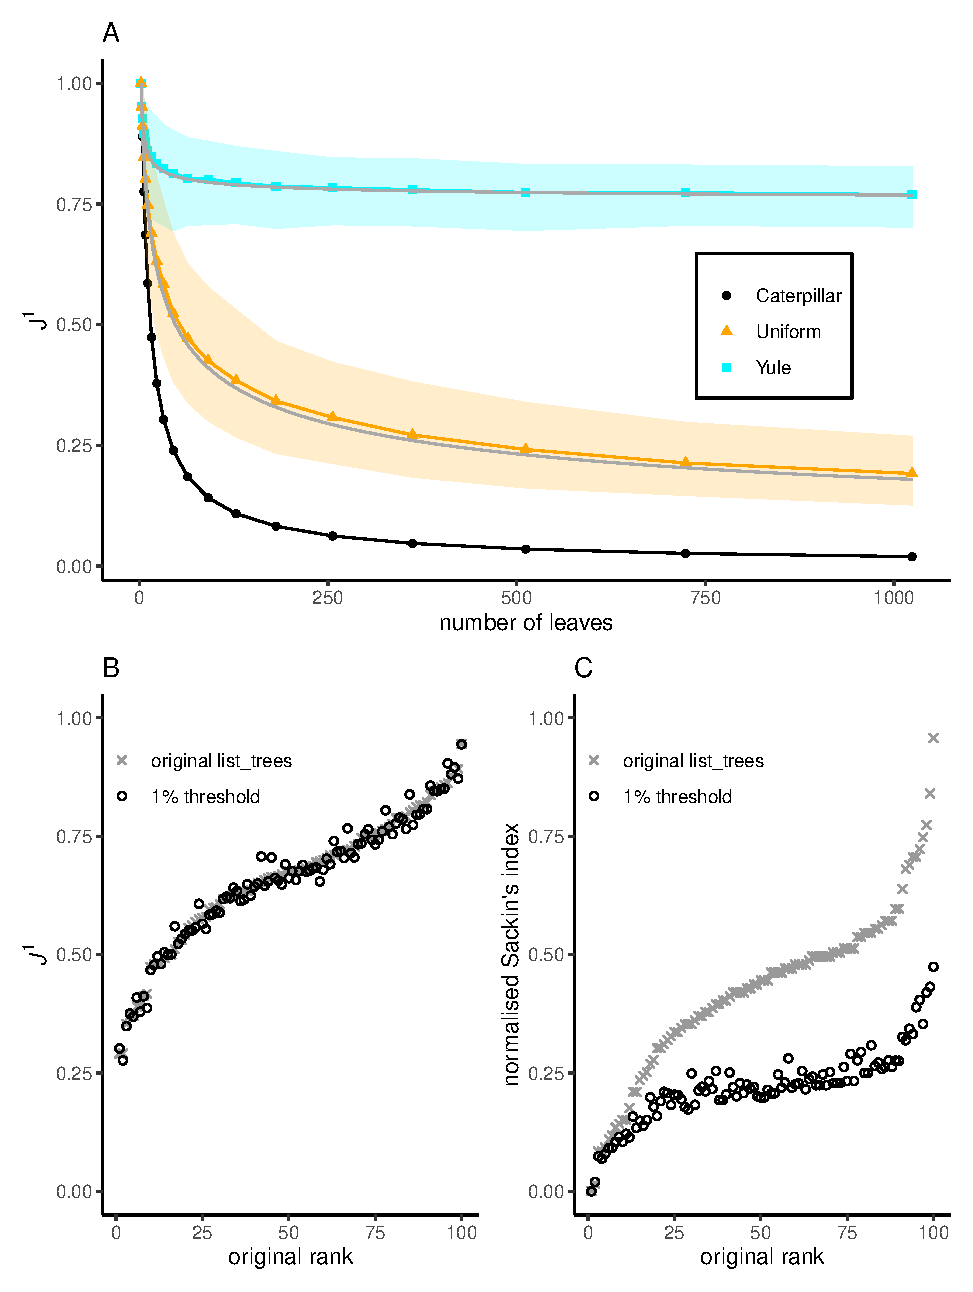
\includegraphics[width=0.82\textwidth]{Chapter_1/figures/old_j1_paper_figure.pdf}
    \caption{\textbf{A} $J^1$ values for trees generated under the Yule process and
    the uniform model. Solid grey curves represent the approximate expected values, and
    the dashed lines the $5$th and $95$th percentiles. \\
    \textbf{B} $J^1$ values for $100$ random
    trees on $16$ leaves using the alpha-gamma model, with $\alpha\sim \text{Unif}(0,1)$
    and $\gamma\sim \text{Unif}(0,\alpha)$. The values were
    calculated before and after applying a $1\%$ population threshold, i.e. removing all leaves
    with sizes smaller than $0.01$ times the total population.\\
    \textbf{C} Normalised Sackin index values for the same trees as in \textbf{B}.}
    \label{fig:robustness}
\end{figure}
\clearpage


\section{Agent-based modelling in oncology}

\subsection{Introduction}
Agent-based models (ABMs) are a class of computational models that simulate the actions and interactions of individual
agents within a system. These agents can represent anything from cells in a tissue to animals in an ecosystem. ABMs
are particularly useful in cancer research, as they can capture the complex interactions happening on the microscale in
cancer. Spatial agent-based models (SABMs) are a subclass of ABMs that incorporate spatial information into the
simulations. This is particularly useful for modelling solid tumours as it allows for the simulation of things like
the spatial heterogeneity of the tumour microenvironment and the effects of spatial constraints on tumour growth.
A strength of ABMs is that they can be as simple or as complex as the researcher needs them to be \cite{colyer_seven-step_2023}.
However, therein lies their weakness, as oversimplification of a model can lead to rapid loss of its utility in
capturing the behaviour of a complex system such as cancer. On the other hand, a model that is too complex, and
attempts to include everything from epigenetic mutations to the effects of the immune system on the tumour, is likely
too computationally expensive to be useful for modelling a tumour of reasonable size. This is an organic demonstration
of many a researcher's favourite saying \textit{all models are wrong, but some are useful, and some are more useful
than others}. In parsing through the literature and developing a new model of our own, we have also been influenced
by an alternative wording of this, that is \textit{the best model is its own worst enemy}, by Philip Maini. Our
interpretation is that a good model should address the questions it was designed to answer, but also open up new
ones which require further investigation, improvements, and research. For example, one can use our demon-warlock
framework \cite{bak_warlock_2023} to simulate the evolution of a tumour in space and draw conclusions on how
spatial organisation will impact intratumour heterogeneity or patient outcomes \cite{noble_when_2020, noble_spatial_2022}.
However, the model does not address the impact of the immune system, spatial heterogeneity in the microenvironment,
or the effects of therapy without further modifications. Alternatively, we may want to include diffusion of
nutrients and waste products in the model, or the effects of hypoxia on the tumour cells. Tools that would be
appropriate for such tasks are, for example, HAL \cite{bravo_hybrid_2020} or PhysiCell \cite{ghaffarizadeh_physicell_2018},
but they are not ideal either as simulating a realistically-sized tumour with these models is prohibitively expensive
in terms of computational resources. Thus, our preferred approach is to develop a proprietary model which is
informed by the literature and the data, and which has ample room for future expansion and improvement.

\subsection{The \texttt{demon-warlock} framework}
In a recent paper \cite{bak_warlock_2023}, we formally introduced a new agent-based model for simulating the
evolution of a tumour in space. The model is designed to be versatile and able to simulate a wide range of
spatial configurations and evolutionary properties of cancer. Spatially, the model is based on a 2D grid, where
each grid cell represents a deme, that is a spatially homogeneous population of cells. Each cell in the model
belongs to a genotype, a unique identifier based on the cell's mutations, and a driver genotype, which differentiates
itself from the genotype by not taking into account passenger mutations. Cell migrations in the tumour have multiple
modes, including invasion of tissue and other demes, and deme fission. The latter allows for the simulation of
tumours with a glandular structure, such as colorectal cancer. Events in the model are scheduled according to the
Gillespie algorithm, with the event hierarchy shown in figure \ref{fig:demon_events}. As the model was written
predominantly in plain C, it is highly efficient considering the complexity of the simulations it can run. An
accompanying R package, \texttt{demonanalysis}, is available for the analysis and visualisation of the model's
output, e.g. figure \ref{fig:demonanalysis_example}. \par
Despite the model's versatility, it is not without its limitations. In its current form, it is not feasible to
simulate tumours larger than a few million cells. This leaves out the possibility of simulating realistically-sized
glandular tumours which can contain a few million glands containing thousands of cells each at the time of diagnosis.
Furtermore, as the main limitation of the model's scalability is tied to the inherent inefficiency of generating
random numbers, it is not well-suited to simulating neutral stochastic markers, such as fluctuating methylation
clocks \cite{gabbutt_fluctuating_2022}. This is further discussed in section \ref{section:old_famework}.

\begin{figure}[h]
    \centering
    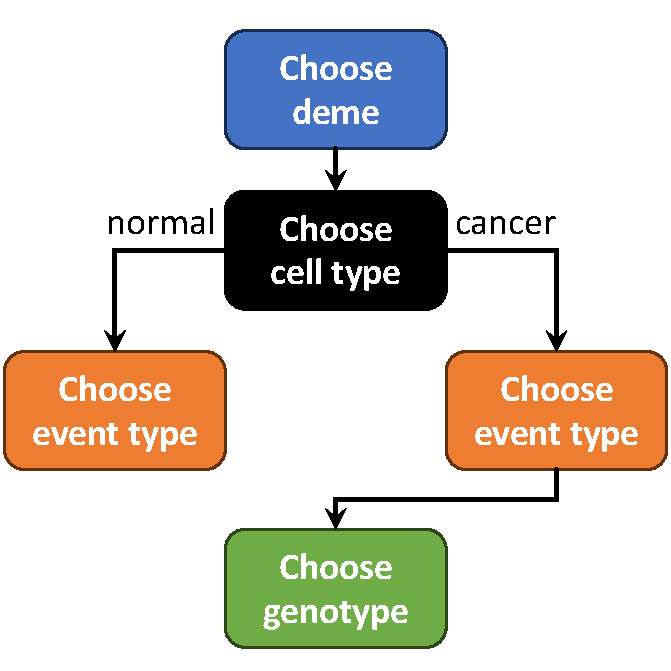
\includegraphics[width=0.75\textwidth]{Chapter_1/figures/demon_hierarchy.pdf}
    \caption{Event hierarchy in the \texttt{demon-warlock} framework. Figure reproduced from \cite{bak_warlock_2023} with
    the authors' permission.}
    \label{fig:demon_events}
\end{figure}

\begin{figure}[h]
    \centering
    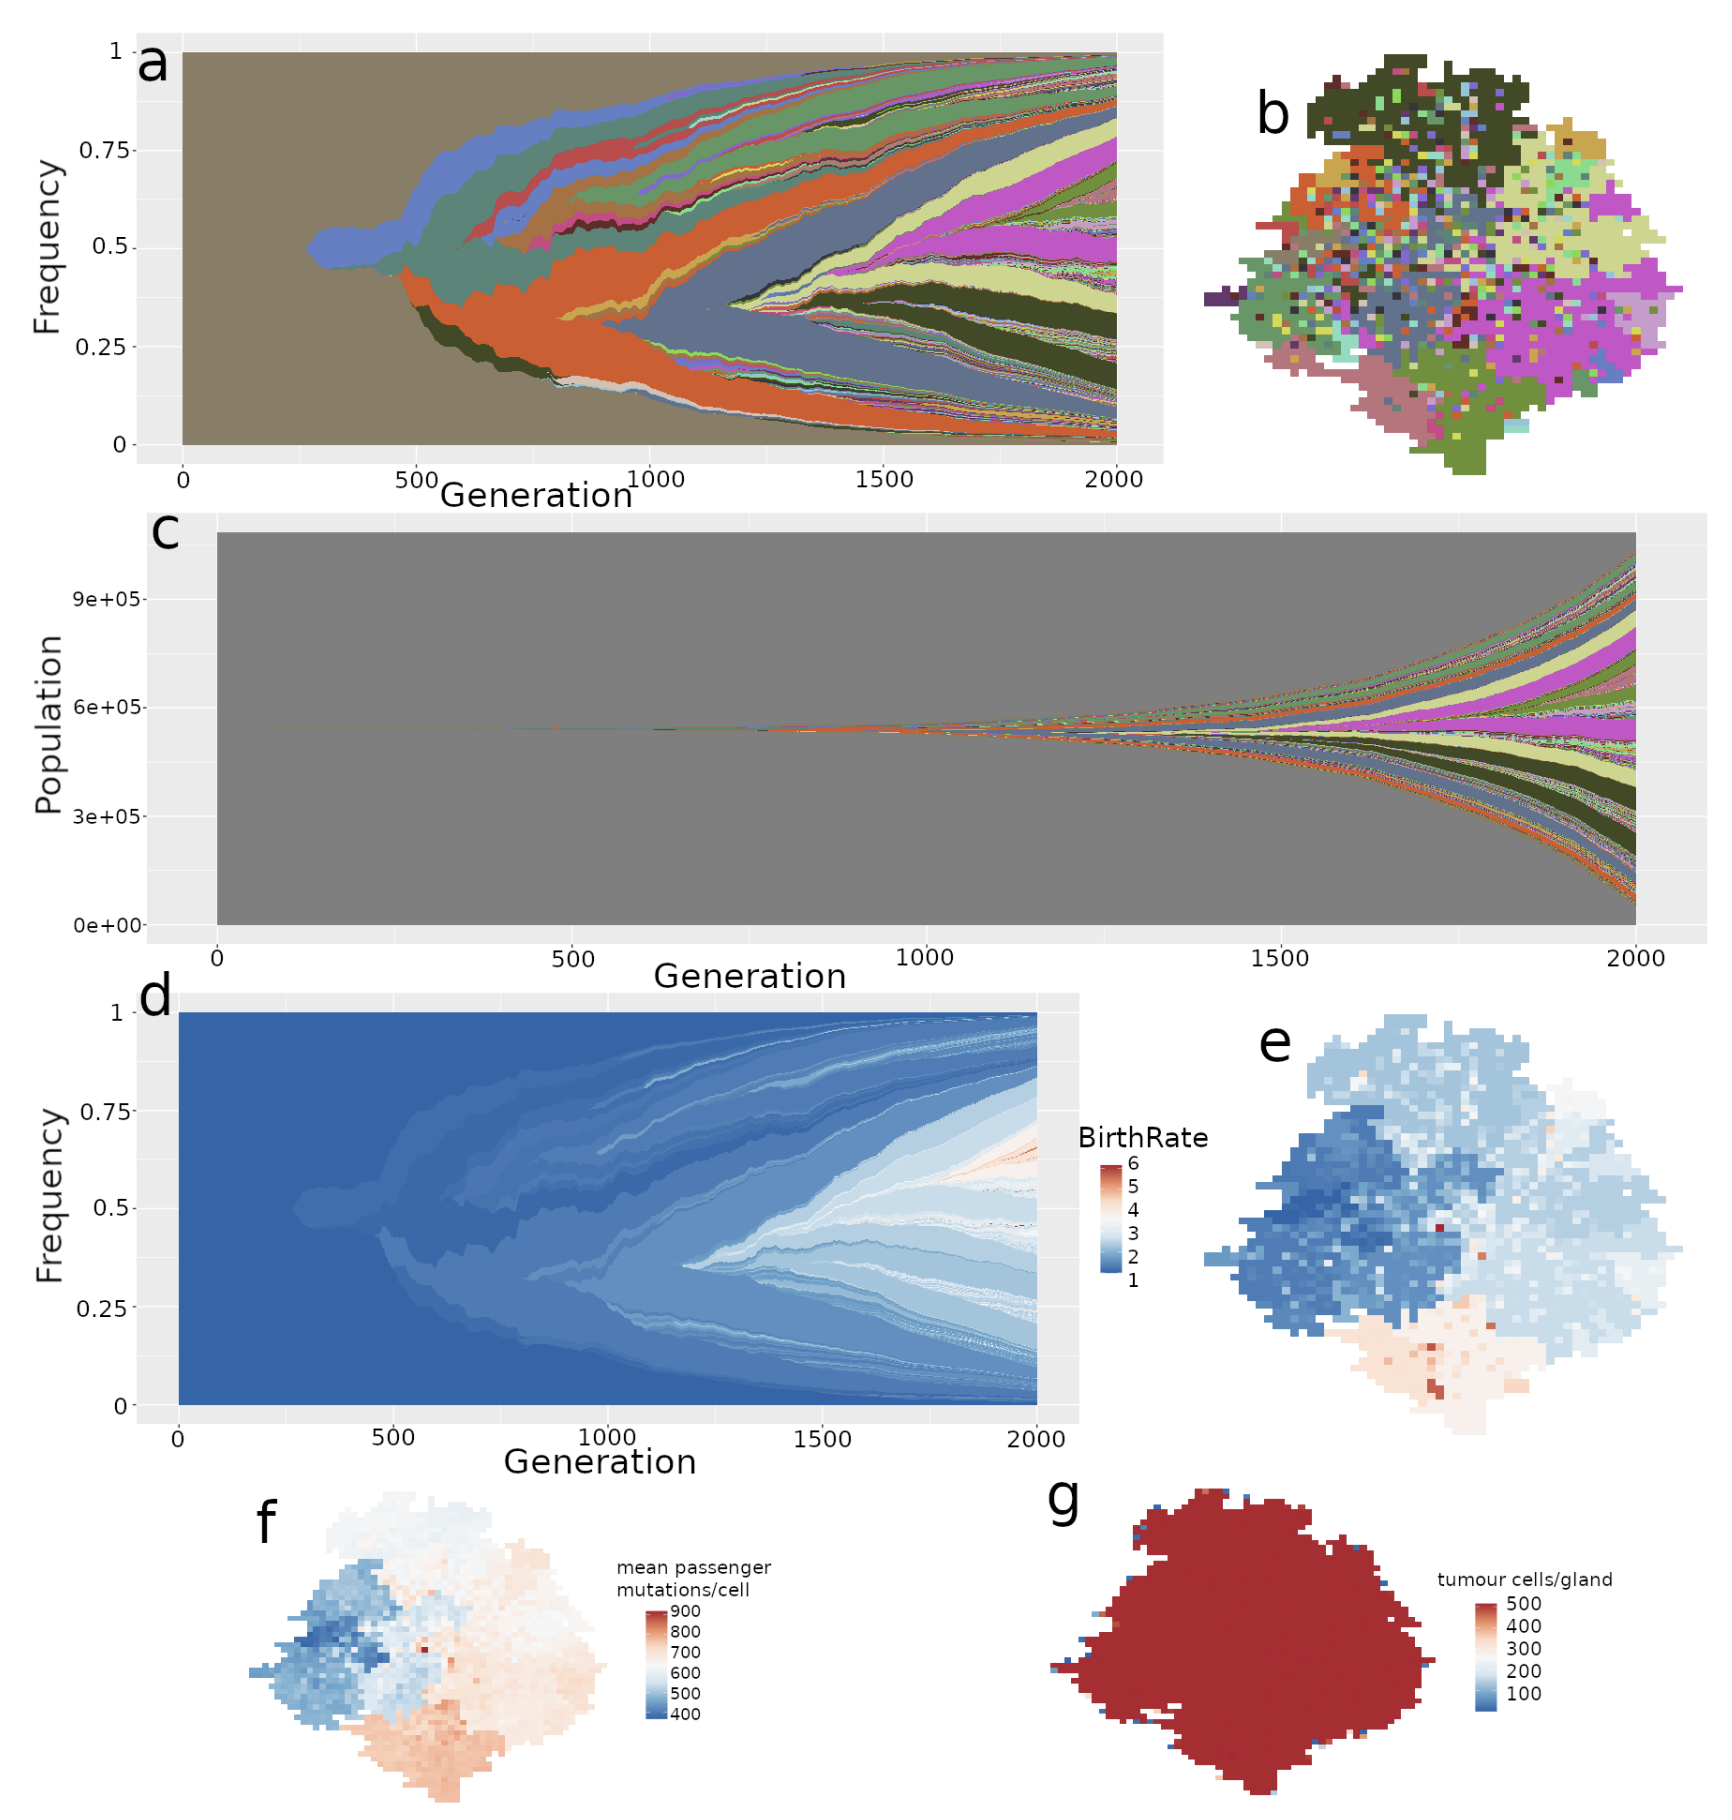
\includegraphics[width=\textwidth]{Chapter_1/figures/demonanalysis_example.png}
    \caption{Example output from \texttt{demon}, visualised using the \texttt{demonanalysis} package.
    \textbf{a} Muller plot of clonal dynamics over time. Each colour represents a clone with a distinct
    combination of driver mutations.
    \textbf{b} Final proportions and spatial plot of clones.
    \textbf{c} Fish plot of clone populations over time using the same colours as in \textbf{a}.
    \textbf{d} Muller plot showing evolution of tumour cell division rate.
    \textbf{e} Final spatial distribution of cell division rates.
    \textbf{f} Final spatial distribution of the mean numbers of passender mutations per cell.
    \textbf{g} Final spatial distribution of the number of tumour cells per gland.}
    \label{fig:demonanalysis_example}
\end{figure}
\clearpage

\section{Likelihood-free inference}
\subsection{Introduction}
To verify whether a model predicts behaviour of the observed system, a common approach is comparing its
output to measurements. The way this is done depends on the complexity of the model and the data. Here
we discuss the general framework of likelihoo-free inference, and more specifically the use of Approximate
Bayesian Computation (ABC). \par
Models based on differential equations can be compared to data using likelihood-based methods. In the
frequentist tradition, the likelihood function is used to estimate the parameters of the model under the
assumption that there is a correct, or ``true" value of those parameters. An alternative approach is
Bayesian statistics, which uses random variables ($\theta$) to represent the uncertainty in the parameters. The
distribution of these random variables before observing the data is called the prior distribution ($P(\theta)$).
After performing measurements in the system and obtaining data ($D$) which has an associated likelihood function
($P(D|\theta)$), the prior distribution is update to the posterior distribution ($P(\theta|D$)) using Bayes' theorem
\cite{bayes_essay_1763}:
\begin{equation}
    P(\theta|D) = \frac{P(D|\theta)P(\theta)}{P(D)}
\end{equation}
The likelihood function is thus a key component of Bayesian statistics, quantifying the probability of observing
the data given the parameters of the model. However, its greatest asset is also its greatest weakness. Depending
on the complexity of the model and the data, the likelihood function can be difficult or impossible to calculate
analytically, or can be too computationally expensive to calculate numerically. This is especially true for
stochastic models, such as agent-based models, where the likelihood function is often intractable. \par
In the case of intractable likelihoods, a common approach is to use likelihood-free inference methods, designed
to approximate the posterior distribution without the need to calculate the likelihood function. These methods
rely on the generation of simulated data from the model, and the comparison of these simulations to the observed
data. Instead of calculating the likelihood fucntion, these methods often involve a process of simulation and
rejection. A common drawback of likelihood-free inference methods is that they can be computationally expensive,
as they often require a large number of simulations to obtain a good approximation of the posterior distribution.
However, as the computational power of modern computers increases, these methods are becoming more and more
feasible for a wide range of models and data.

\subsection{Approximate Bayesian Computation}
Approximate Bayesian Computation (ABC) is a likelihood-free inference method that has gained popularity in the
last three decades \cite{tavare_inferring_1997, lechevallier_integrating_2010, jagiella_parallelization_2017}.
The basic idea behind ABC is to approximate the posterior distribution of the parameters of a model by comparing
simulated data to observed data. \par
In the most general form of ABC, the algorithm proceeds as follows:
\begin{enumerate}
    \item Sample a set of parameters from the prior distribution, $\hat\theta$.
    \item Simulate data from the model using the parameters.
    \item Compare the simulated data ($\hat D$) to the observed data ($D$) using a distance function, $d(\hat D, D)$.
    \item If the distance between the simulated and observed data is less than a certain threshold $\epsilon$, accept the
    parameters. Otherwise, reject them.
    \item Repeat steps 1-4 until a sufficient number of accepted parameters have been obtained.
\end{enumerate}
The distance threshold must be strictly positive, and is often chosen to be a small value. The choice of the distance
function is crucial, as it determines how the simulated data is compared to the observed data. Alternatively, in the
case of high-dimensional data, the distance function can be replaced by a summary statistic, $S$, which is a function of the
data, i.e. $d'(S(\hat D), S(D))$. The choice of summary statistics is also crucial, as it determines how the data is
reduced before the comparison. \par
ABC does not come without its own set of challenges. As it relies on comparing relevant features of the simulated data to
the observed data, the choice of summary statistic or distance metric is crucial, as it determines how the data is
reduced before the comparison. Fortunately, there are methods for reducing dimensionality of the data which
narrows in on its informative aspects \cite{blum_comparative_2013}.
The choice of the distance threshold is also essential, as it determines
the acceptance rate of the algorithm. Setting the threshold too high or too low can lead to biased or inefficient
estimates of the posterior distribution. However, this can be mitigated by using a dynamic threshold, which is
adapted during the course of the algorithm \cite{prangle_adapting_2017}.
Finally, the computational aspects of ABC must be mentioned, as the algorithm relies on repeated simulations of
potentially complex models. This can require a large amount of computational resources, raising questions about
the method's scalability and practicality. An obvious way to circumvent this is to use a model which is as
lightweight as possible. Even in the case of infinite compute available, one must be mindful of the fact that
the more complex the model, the more complex the inference problem, and the more complex the inference problem,
the more complex the model. This is a feedback loop which can render both the model and subsequent analysis
uninterpretable. Therefore, we believe that the best practice as a mathematician and applied scientist is to abstract
the model enough to be able to draw conclusions from it, but not so much that it becomes uninformative. \par
In chapter \ref{chapter:methdemon}, we introduce our simplified model of colorectal cancer gland fission and
the accompanying ABC workflow. We discuss the choice of summary statistics and the performance of the ABC
algorithm, and subsequently demonstrate the model's utility in inferring the evolutionary history of a tumour
from methylation data in chapter \ref{chapter:methylation}.


\section{Fluctuating methylation clocks}
The concept of a molecular clock is a hallmark of evolutionary biology. It is based on the idea that the
rate of evolution of a particular gene or set of genes is constant over time, and can be used to estimate
the time of divergence between species or the time of a particular event in the evolutionary history of a
species. The most famous example of a molecular clock is the mitochondrial DNA clock, which is used to
estimate the time of divergence between species \cite{hasegawa_dating_1985}. The key principle behind molecular
clocks is that closely related species or individual will have more similar sequences than distantly related
ones. This also translates to individual cells in cancer. The issue with using molecular clocks in cancer
is that ``slowly ticking" molecular clocks, i.e. ones with a low mutation rate, are not informative enough
on the timescale of cancer evolution, limiting their utility to cell lineages which diverged too far in the past,
with recent events remaining undetectable. On the other hand, ``fast ticking" molecular clocks can
reveal recent evolutionary events but also have their own limitations, such as independent mutations in the
same site \cite{kuipers_single-cell_2017}. \par
\textit{TO DO:} Introduce and discuss FMCs.



\section{Aims and objectives}

\subsection{Hypotheses}
\begin{enumerate}
    \item The $J^1$ index is a universal measure of tree balance, and can be used, in conjunction with other
        tree shape indices, to differentiate between evolutionary modes in cancer.
    \item Spatial agent-based models are a powerful tool for simulating the evolutionary dynamics of solid tumours.
    \item These methods are useful for inferring the evolutionary history of colorectal cancer based on multi-site
        methylation array sequencing.
\end{enumerate}

\subsection{Aims}
\begin{enumerate}
    \item Calculate or approximate important properties of the $J^1$ index, such as its expected value under
        standard tree-generating processes.
    \item Determine the utility of sets of tree shape indices for differentiating between evolutionary modes in cancer.
    \item Extend the fluctuating methylation clock model to multi-site sequencing of solid tumours on the
        example of colorectal cancer.
\end{enumerate}

\subsection{Objectives}
\begin{enumerate}
    \item Contextualise $J^1$ within the broader field of tree shape indices in biology and computer science.
    \item Investigate extreme and expected values of $J^1$ under standard tree-generating processes.
    \item Recapitulate the classification of evolutionary modes in cancer using a set of three tree shape indices.
    \item Extend the discussion to a more interpretable and general system of tree shape indices.
    \item Develop an agent-based model for simulating the evolutionary dynamics of colorectal adenocarcinoma.
    \item Develop an ABC workflow for inferring the evolutionary parameters of the model, specifically the
        gland fission rate, methylation and demethylation rates, driver mutation rate, selective advantage,
        and the effective number of lineages per tumour gland.
    \item Apply the model to colorectal cancer data and compare the inferred phylogenies to the trees generated
        by the model.
\end{enumerate}


\chapter{Extreme and expected values of universal tree balance index $J^1$}\label{ch_trees}
\textbf{TO DO: } Finish introductions
\section{Introduction}
	%\begin{itemize}
	%    \item literature review - tree methods through the ages and relevant questions in cancer evolution
	%    \item discussion of the balance index paper - go through the discussion and identify points which can be expanded, use it as inspiration for the indtroduction
	%\end{itemize}
 %TO DO: introduce weight balance trees and discuss the similarities between them and the trees we use for J^1
%- intro: explain what tree balance is and why it's useful, add references to papers using/explaining tree balance in CS and phylo; first few sentences are quite vague, can be cut if not all that important
- there are different ways to define tree balance, depending on field and, consequently, type of tree\\
- however, it is an important concept \textbf{*explain what it means for data structures and phylogenetics*}\\
- explain how evolutionary process differences can affect tree balance and mention the problem of phylogenetic trees in cancer\\
The balance of a tree can imply properties other than the symmetry in the tree's topology. Depending on the choice of index from at least $19$ available in literature \cite{fischer_tree_2021}, the intuition and results may vary drastically or not at all between them. A common issue among them, however, is universality --- some indices are only defined under certain topological restrictions (such as bifurcating trees), while others may not account for trees containing internal nodes with only one descendant or nodes with non-zero node sizes. As a consequence, it is difficult to use one index across different areas of research or even compare trees on different numbers of leaves from the same data source. Having a universal measure of balance applicable in this way would enable sensical comparison between any two trees. \par
In phylogenetics, balanced trees 
In a previous paper \cite{lemant_robust_2021}, we introduced a new robust, universal balance index $J^1$. This index can be used on any tree topology and can account for trees whose nodes have non-zero size. The basic properties of the index are covered in the original paper, and in this follow-up we explore additional questions one might have when choosing a balance index.


\section{Definitions}\label{defsec}
Before getting into the properties of $J^1$ and related indices, we will briefly introduce these indices, tree naming suggestions and conventions, and notation used throughout the paper. 
\begin{definition}[Rooted tree]
    A \textbf{rooted tree} $T$ is a connected acyclic graph with node set $V(T)$, edge (branch) set $E(T)$, and node magnitudes assigned from $\mathbb{R}^+_0$, with an internal node designated as the root of $T$. We denote with $\tilde{V}(T)$ the set of nodes with descendants of non-zero magnitude of tree $T$ and with $L(T)$ the set of its leaves, that is nodes with no descendants.\\
    A \textbf{leafy tree} is a tree whose leaves are of equal non-zero size, and all internal nodes have size zero.
\end{definition}
\begin{remark}
	In general, a tree can have associated edge (or branch) lengths. We do not discuss such trees in this paper but focus on trees with equally sized branches.
\end{remark}
\begin{definition}[The Sackin index]
    Let $T$ be a rooted bifurcating tree on $n$ leaves. We define the \textbf{Sackin index} of tree $T$ as the sum of distances of the tree's leaves from its root i.e., 
    \begin{equation}\label{sackindef}
        I_S = \sum_{l\in L(T)} \nu(l),
    \end{equation}
    where $\nu(l)$ is the depth of leaf $l$.
\end{definition}
\begin{remark}
    The Sackin index can be generalised for trees with arbitrary node degree distributions. In this case, it is calculated as 
    \begin{equation}\label{gensackindef}
        I_{S,\text{gen}} = \sum_{i\in V(T)} S_i^*,
    \end{equation}
    where $S_i^*$ is the size of the subtree rooted in internal node $i$, excluding node $i$. 
\end{remark}
\begin{definition}[Robust balance index]
            The robust balance index $J^1$ of tree $T$ is calculated as
            \begin{equation}\label{J1def}
                J^1(T) = \frac{1}{\sum_{l\in\tilde{V}}S_l^*} \sum_{i\in\tilde{V}} S_i^{*}\sum_{j\in C(i)}W_{ij}^{1},
            \end{equation}
            where $S_i^*$ is the magnitude of the subtree rooted in node $i$, $C(i)$ is the set of direct descendant nodes of node $i$, and $W_{ij}^1$ is the node balance function defined as 
            \begin{equation}\label{Wij1}
                W_{ij}^1 = 
                \begin{cases}
                    -\frac{S_j}{S_i^*}\log_{d^+(i)}\frac{S_j}{S_i^*},& \text{ for } d^+(i);\\
                    0, & \text{ otherwise,}
                \end{cases}
            \end{equation}
            where $S_i$ is the magnitude of the subtree rooted in node $i$, including node $i$, and $d^+(i)$ is the out-degree of node $i$.
\end{definition}
\begin{definition}[Cherry]
	A tree consisting only of a root and two leaves is called a \textbf{cherry}.
\end{definition}
\begin{definition}[Yule model \cite{yule_iimathematical_1925}]\label{yuledef}
    Consider a bifurcating tree $T$ on $n$ leaves. To obtain the probability of generating $T$ under the Yule model, start with a single node and replace it with a cherry. Then, at each step, choose one leaf uniformly at random and replace it with a cherry, until the tree has $n$ leaves. The sum of probabilities of generating $T$ in all possible ways is the probability of generating $T$ under the Yule model.
\end{definition}
\begin{definition}[Uniform model \cite{rosen_vicariant_1978}]\label{unifdef}
    Under the \textbf{uniform model} of tree generation, every bifurcating tree on $n$ leaves has an equal probability of being generated, which is equal to $n\binom{2n-2}{n-1}^{-1}$.
\end{definition}
\begin{remark}
	We only consider leafy trees with equal leaf magnitudes in definitions \ref{yuledef} and \ref{unifdef}.
\end{remark}

\begin{figure}[h!]
    \centering
    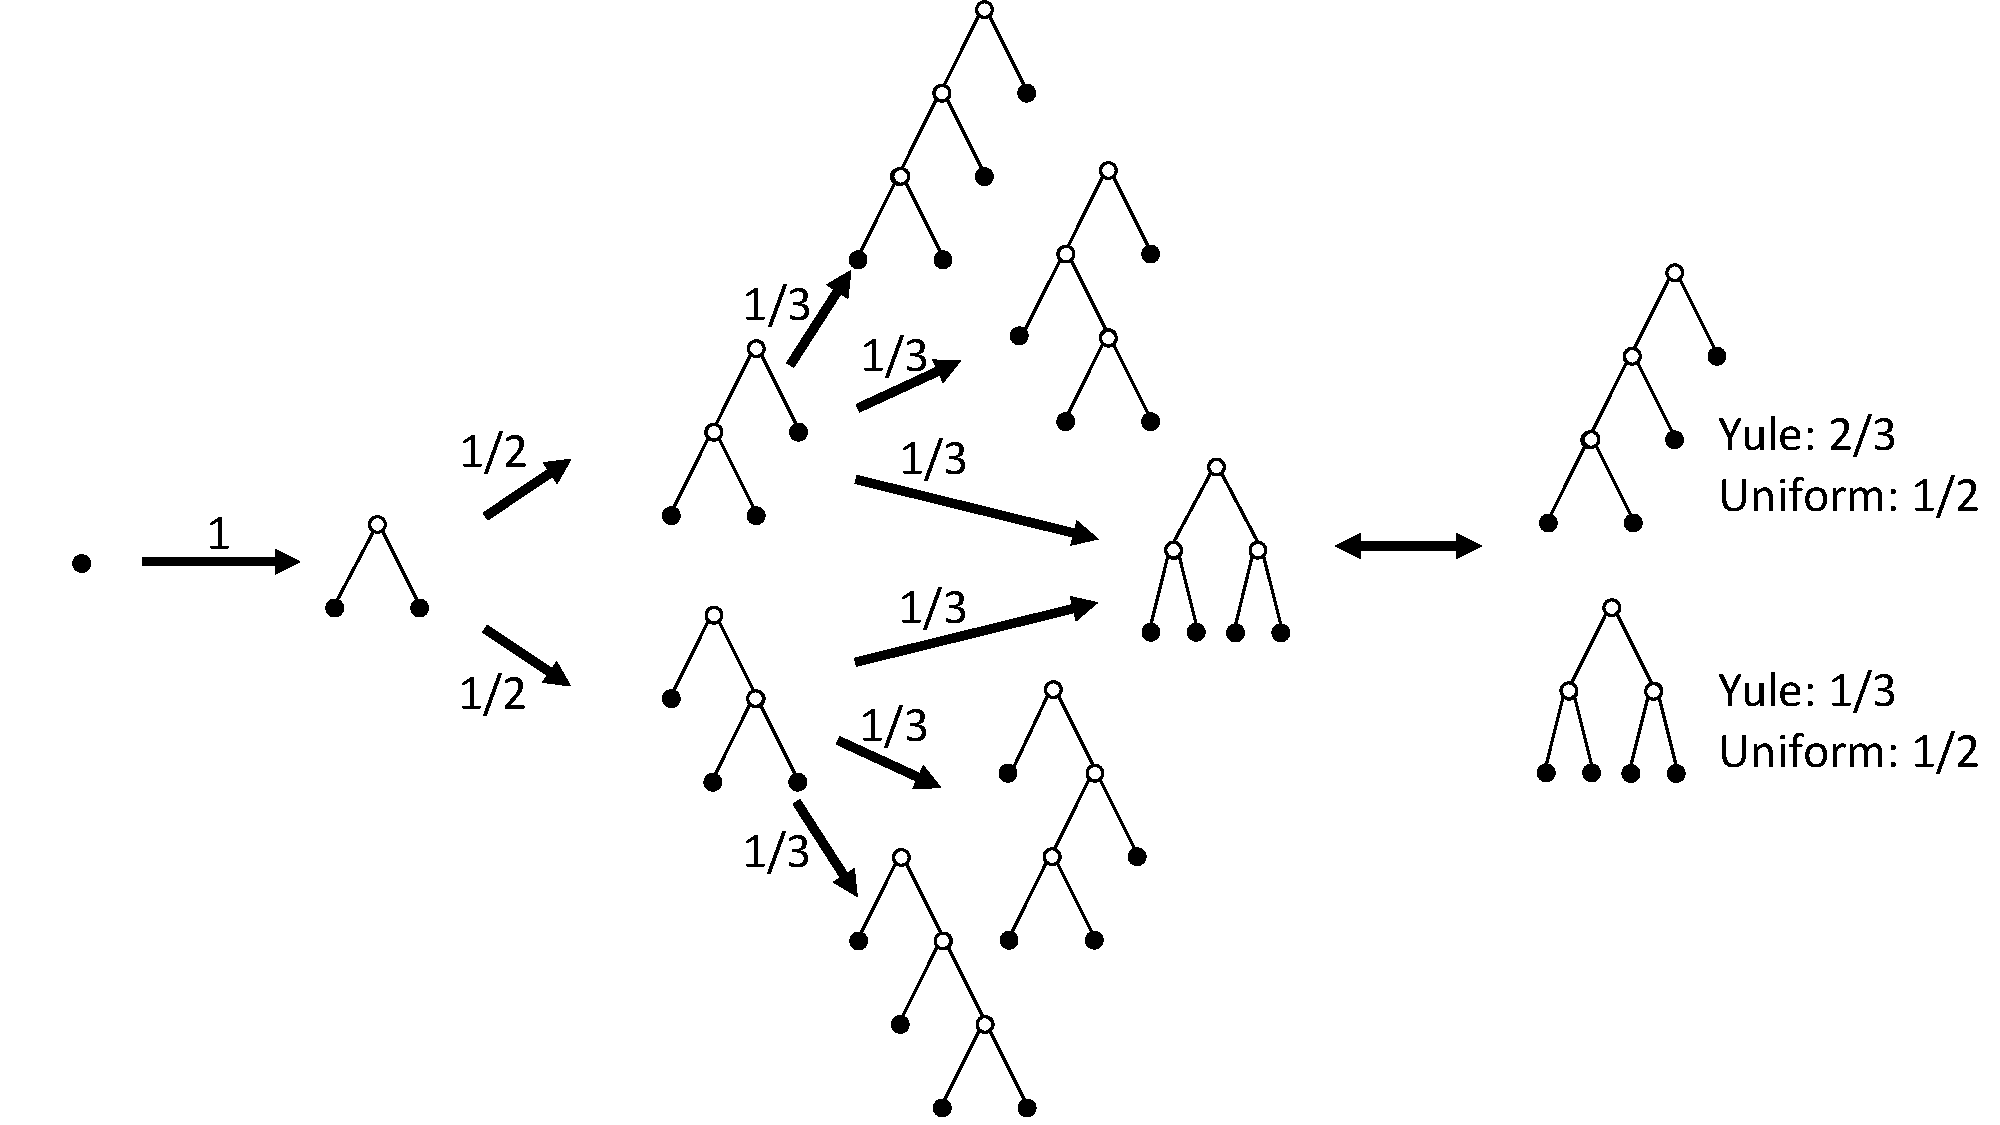
\includegraphics[width=\textwidth]{Chapter_trees/figures/yule-unif-figure.pdf}
    \caption{Comparison of probabilities for generation of trees on $4$ leaves under the Yule and uniform models.}
    \label{yule-unif-figure}
\end{figure}

The Yule and uniform models are statistical models which find their applications in evolutionary biology. Specifically, the Yule model, also known as the pure birth and coalescent model, is used when considering speciation rates and patterns \cite{aldous_stochastic_2001, steel_properties_2001}. The uniform model is typically encountered in evolutionary process considerations \cite{mooers_inferring_1997, steel_distributions_2000}. While simple, the two are are valuable null models for studying different aspects of evolution.


\section{Balancing binary trees according to $J^1$}
The balance index $J^1$ is defined on trees with arbitrary node out-degree distributions and node magnitudes \cite{lemant_robust_2021}. Depending on use case, this definition may be considered too broad. Specifically, in computer science the most commonly used tree is a binary tree.

\begin{definition}[Binary tree \cite{nievergelt_binary_nodate}]
	A \textbf{binary tree} is a rooted tree such that each node can have $0$, $1$, and $2$ children.
\end{definition}

While $J^1$ originally draws inspiration from the problem of quantifying properties of cancer phylogenetic trees \cite{noble_spatial_2022}, trees are encountered and used regularly in other fields, such as the broader realm of evolutionary biology, as well as computer science. However, one might notice that the notion of balance is used differently across those fields, being an effectively binary consideration in data structures, i.e. a tree can be balanced or unbalanced based on some measure \cite{nievergelt_binary_nodate}. In evolutionary biology, a finer scale is used, and comparisons between trees are more relevant \cite{mir_new_2013, mir_sound_2018, fischer_tree_2021}. Despite these differences, we have shown robustness of our method under common data gathering errors in biology \cite{lemant_robust_2021} and can further show that it generalises tree balance in data structures. Let us begin by defining the different measures of balance encountered in computer science literature.

\begin{definition}[Root balance score]
    The \textbf{root-balance score} $\rho(T_n)$ of a binary tree $T_n$ on $n > 1$ nodes is
    \begin{equation}\label{defrootbalscore}
        \rho(T_n) = \frac{l+1}{n+1},
    \end{equation}
    where $l$ is the number of nodes in the left subtree of $T_n$.
\end{definition}
Intuitively, one could imagine the root balance score as evaluating how well the tree could be balanced on a fulcrum placed under node $n$.

\begin{definition}[Weighted path length]
    Let $T$ be a rooted tree on $n$ nodes, and $\alpha_i$, $i=1,2,...$ the weights (or access frequencies) assigned to its nodes $v_i$. We define the \textbf{weighted path length} of tree $T$ as
    \begin{equation}\label{wpathdef}
        |T_n| = \sum_{v_i \in V(T)} \alpha_i \nu(v_i).
    \end{equation}
\end{definition}


\begin{remark}
    Let us rewrite the weighted path length in a more familiar way:
    \begin{equation*}
        |T| = \sum_{v_i \in V(T)} \alpha_i \nu(v_i) = \sum_{i \in V(T)} p_i \nu(i) = \sum_{i\in V(T)} S^*_i,
    \end{equation*}
    which is just the generalised Sackin index for tree $T$. 
\end{remark}
Consider then the following proposition.
\begin{proposition}[Lemant et al. \cite{lemant_robust_2021}]
    Let $T$ be a leafy tree on $n$ leaves with $d^+(i) = m > 1$. Then
    \begin{equation}
        J^1(T) = \frac{n\log_mn}{I_S(T)} \label{prop6}
    \end{equation}
    where $I_S$ is the Sackin index.
\end{proposition}
%state as a proposition and write down a brief proof properly - need to introduce proposition 6 before this happens also, could be a corollary
\begin{corollary}
    We can rewrite equation \eqref{prop6} for binary trees as 
    \begin{equation}
        J^1(T) = \frac{n\log_2n}{|\bar{T}|}. \label{corr6}
    \end{equation}
    This means that, for a fixed number of leaves $n$, minimising the weighted path length $|\bar T|$ is equivalent to maximising $J^1$. 
\end{corollary}

\begin{theorem}[Nievergelt and Wong \cite{wong_upper_1973}]
    Let $T_n$ be a binary node-tree with $n$ nodes and root balance score $\beta$. Then its total path length $|T_n|$ is bound from above by
    \begin{equation}\label{path_upper_bound}
        |T_n|_\text{upper} = (H(\beta))^{-1}(n+1)\log_2(n+1)-2n,
    \end{equation}
    where $H(\beta) = \beta\log_2\beta^{-1}+(1-\beta)\log_2(1-\beta)^{-1}$.
\end{theorem}

\begin{corollary}\label{j1_lower_bound_cor}
    There is a lower bound on $J^1$ for binary trees with $n$ nodes and root balance score $\beta$, and it equals
    \begin{equation}\label{j1_lower_bound}
        J^1_\text{lower} = \frac{n\log_2n}{|T_n|_\text{upper}}.
    \end{equation}
\end{corollary}

Corollary \ref{j1_lower_bound_cor} follows trivially from proposition \ref{j1_lower_bound} but represents a result which has a deeper connection to the fundamentals of information theory.

\begin{proposition}
    The Huffman method \cite{huffman_method_nodate} maximises $J^1$ on binary trees for a given set of node magnitudes.
\end{proposition}
\begin{proof}
    Consider a set of non-negative real numbers $F = \{\alpha_1, \dots, \alpha_m\}$. The Huffman method places larger numbers, i.e. nodes of higher magnitude, closer to the root, minimising the weighted path length as a result. By corollary \ref{j1_lower_bound_cor}, the Huffman method maximises $J^1$.
\end{proof}
As Huffman coding is an optimisation algorithm, we can use $J^1$ to measure how close a tree constructed using a given set of node magnitudes is to the maximally balanced binary tree on the same set. This means one can meaningfully measure how close an alternative algorithm which runs in a faster time complexity, such as arithmetic coding \cite{pasco_source}, gets to the optimal solution.

Let us now define the most common binary tree type one might encounter in computer science literature, binary search trees.
\begin{definition}[Binary search tree]
    A \textbf{binary search tree} $T_n$ over $n$ entries (w.l.g. numbers) $x_1,\dots,x_n$ is a labelled binary tree, each of whose nodes have been labelled with a distinct number chosen from $x1,\dots,x_n$ such that for each node $N$, all nodes in the left subtree of $N$ have a smaller $x_i$ as their label than $x_N$, and all nodes in the right subtree of $N$ have a larger number as their label than node $N$.
\end{definition}
The balance of binary search trees is usually measured by comparing the numbers of leaves in the left and right subtrees of the root. A more specific use case of binary search trees is for implementing dynamic data structures such as dictionaries \cite{tsakalidis_maintaining_1984}. For this purpose, weight-balanced trees are often used.
\begin{definition}[Weight-balanced tree]
    A weight-balanced tree is a binary search tree that stores the sizes of subtres in the nodes. That is, a node contains:
    \begin{itemize}
        \item key, of any type;
        \item value;
        \item left and right pointers to the child nodes;
        \item size.
    \end{itemize}
\end{definition}
\begin{definition}[Node balance]
    A node $i$, with children $i_l$ and $i_r$ and corresponding weights $w[i], w[i_l], w[i_r]$, is $\alpha$-weight-balanced if 
    \begin{align}
        w[i_l] \geq & \alpha w[i], \label{weight-balance-left} \\
        w[i_r] \geq & \alpha w[i], \label{weight-balance-right}
    \end{align}
    where $\alpha$ is a numerical parameter to be determined when implementing weight-balanced trees.
\end{definition}
Recall the general definition of $J^1$, where each internal node has an associated node balance. In the most general definition of $J^1$, equation \eqref{J1def}, the node balance $W_i$ of node $i$ can be any function $W_i: \mathbb{N}\to\mathbb{R}_{\geq 0}$ according to some property of node $i$ and its descendants. In other words, one may consider the node balance score $W_i$ as a generalisation of the root balance score since it calculates how evenly a node's descendants split the subtree rooted in it, as opposed to the overall tree structure. \par

The balance of weight-balanced trees is optimised dynamically through operations called rotations, which keep the weights of left and right subtrees within $\alpha$ of each other. Balance plays a major role in constructing good data structures in computer science, but computational efficiency is of much greater importance in the field, with balancing happening dynamically when new trees are initialised or nodes added to existing ones, other good examples being AVL trees and red/black trees \cite{noauthor_art_nodate}. The role of balance indices for static data structures is thus quite niche. However, by having a mathematically robust definition underpinning $J^1$, and considering general features of rooted trees, we have shown that it can easily be used far wider than just the original application of analysing cancer phylogenies. The connections between different tree use cases thus to show how one can construct powerful methods for general use without sacrificing specificity.

\begin{figure}
    \centering
    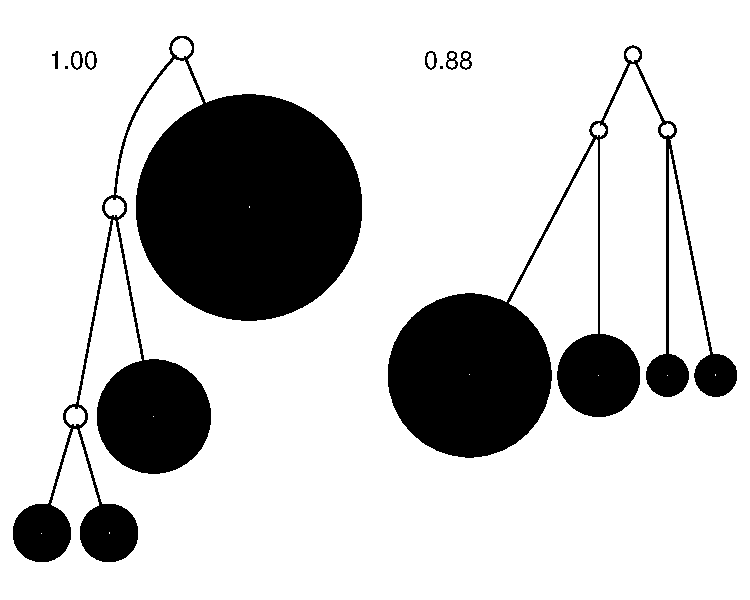
\includegraphics[width=0.8\textwidth]{Chapter_trees/figures/balcat.pdf}
    \caption{By including the node-balance function $W^1$ in $J^1$, we allow for the possibility of perfectly balanced caterpillars (left) and less balanced fully symmetric trees (right) based on the node size distribution in the tree.}
    \label{balcat}
\end{figure}

\iffalse
Since the index $J^1$ is related to Sackin's balance index and the Shannon entropy of a given leafy tree, as shown in our previous work \cite{lemant_robust_2021}, we can examine some further properties which results from this relationship. One of the first consequences of Proposition $6$ from the mentioned paper is that, for full $m$-ary cladograms, only the denominator of $J^1$ depends on the tree topology. That is
\begin{equation}
    J^1(T) = \frac{^1H(T)}{\sum_{i\in\mathcal{L}(T)}p_i\nu(i)\log m}, \label{prop6}
\end{equation}
where $\mathcal{L}(T)$ is the set of leaves of tree $T$, $^1H(T)$ is the tree's Shannon entropy, $m$ is the internal node degree, $\nu(i)$ is the node depth of leaf $i$, and $p_i$ is the weight of leaf $i$. This implies that, for a given set of node sizes and topology restricted to the set of bifurcating trees, $J^1$ is minimised using Huffman coding \cite{huffman_method_nodate}, i.e. clustering the heaviest nodes closest to the root, and letting the lightest ones populate the higher depth places (figure \ref{balcat}). While a straightforward result, it is an important demonstration of the universality of $J^1$. This implies that constructing an optimal search tree for a given set of frequencies will minimise $J^1$. Furthermore, consider the weighted path length of a weighted binary tree $T$, as defined in computer science literature \cite{nievergelt_binary_nodate}. One immediately sees that minimising the weighted path length is equivalent to maximising $J^1$ on leafy trees. These results enable us to compare the balance of completely different trees, as the behaviour of $J^1$ is consistent across the board. \\
If we consider a general weight-balance tree, the discussion is only slightly more complicated. In this context, a measure of balance one would commonly encounter in computer science literature is the weighted path length, calculated as 
\begin{equation}\label{weightedPL}
    |T| = \sum_{i\in V} \nu(i) p_i = \sum_{i\in\tilde{V}}S_i^*.
\end{equation}
The only difference between this metric and the Sackin index is the addition of weights in the more general case of trees with non-zero internal node sizes. This quantity is also the normalising factor of $J^1$ which implies a similar relationship between $J^1$ and $|T|$ to that of $J^1$ and Sackin's index, with the addition of the node balance score to account for even splits among a node's descendants. In fact, one might interpret the node balance score as a loose generalisation of the root balance score for each node,
\begin{equation}
    \rho(T_n) = \frac{l+1}{n+1},
\end{equation}
which is the ratio between the number of nodes in the subtree rooted in the left descendant of node $n$ and the number of nodes in the tree rooted in $n$. Furthermore, one could choose a node balance function based on the root balance but as shown in our previous paper, choosing $W^1$ related to the Shannon entropy gives $J^1$ certain desirable properties, a consequence of which is its relationship with Sackin's index. \par
\fi

        
\section{Expected value of $J^1$ under simple evolutionary processes}\label{expsection}
% proposition: E(J^1) approaches nlog_2n/E(I_S) as n goes to infinity under Yule and/or uniform and then prove, make it more like a mathematical paper with a sequence of propositions and proofs
% key things to add: looking at what happens to the upper bound, specifically in the uniform model case
% calculate limits for the edges of the Jensen gap as n goes to infty
For applications in evolutionary theory, an important property of balance indices is their expected value under an evolutionary process, as it tells us which process drove the tree into its current state. Equivalently to standard calculations in probability, one can obtain the expected value of a balance index by calculating the sum of the products of balance index values with the corresponding probability of the tree shape. 
\begin{definition}
Let process $P$ generate tree $T_i$ with probability $p(T_i)$ for $T_i\in\mathcal{T}_n$. The expected value of index $I_B$ on $n$ leaves under process $P$ is defined as
    \begin{equation}\label{expvaldef}
        \mathbb{E}_P^n(I_B) = \sum_{T_i\in\mathcal{T}_n} p(T_i)I_B(T_i).
    \end{equation}
\end{definition}

While the above definition seems quite general, in practice the generating process can introduce constraints on the set of trees. Two of the simplest, and most widely studied, processes of tree generation are the uniform model \cite{rosen_vicariant_1978} and the Yule model \cite{yule_iimathematical_1925}, which generate bifurcating trees. The expected value of a few indices, and even some higher moments in certain cases, are known for each of these tree generation processes \cite{mir_new_2013, m_coronado_sackins_2020, goh_two_2022}. Among these is the Sackin index, which is useful for our purposes. \par
Under the Yule model, the expected value of the Sackin index for trees on $n$ leaves is
\begin{equation}
    \mathbb{E}_Y^n(I_S) = 2n\sum_{i=2}^n \frac{1}{i},
\end{equation}
as shown in \cite{kirkpatrick_searching_1993}. Consider the relationship between $J^1$ and the Sackin index for bifurcating trees, which is directly derived from equation \eqref{prop6},
\begin{equation}\label{J1ISrel}
    J^1 = \frac{n\log_2 n}{I_S}.
\end{equation}
This means that the expected value of $J^1$ for a tree on $n$ leaves, generated under the Yule model is
\begin{equation*}
    \mathbb{E}_Y^n(J^1) = \mathbb{E}_Y^n(\frac{n\log_2 n}{I_S}) = n\log_2 n \mathbb{E}_Y^n(1/I_S).
\end{equation*}
We can rewrite this equation as
\begin{equation}
    \frac{1}{\mathbb{E}_Y^n(1/I_S)} = \frac{\mathbb{E}_Y^n(J^1)}{n\log_2n},
\end{equation}
which is the harmonic mean of the Sackin index. The harmonic mean under the Yule process is not a standard result in literature, nor have we been able to obtain a closed-form solution for this problem so far. We can, however, compare the harmonic and arithmetic means of $I_S$ by considering the Jensen gap
\begin{equation}\label{JensenGap}
    \mathcal{J}(f, X) = \mathbb{E}[f(X)] - f(\mathbb{E}[X]).
\end{equation}

\begin{theorem}[Liao and Berg \cite{liao_sharpening_2017}]\label{jensen_thm}
    Let $X$ be a one-dimensional random variable with mean $\mu$, and $P(X\in(a,b))=1$, where $\infty\leq a<b\leq \infty$. If $\phi(x)$ is a twice differentiable function on $(a,b)$, and
    \begin{equation*}
        h(x;\nu) = \frac{\phi(x)-\phi(\nu)}{(x-\nu)^2} - \frac{\phi'(\nu)}{x-\nu},
    \end{equation*}
    then
    \begin{equation}
        \inf_{x\in(a,b)}\{h(x;\mu)\}\mathrm{Var}(X) \leq \mathbb{E}[\phi(X)] - \phi(\mathbb{E}[X]) \leq \sup_{x\in(a,b)}\{ h(x;\mu) \}\mathrm{Var}(X).
    \end{equation}
\end{theorem}

\begin{proposition}\label{jensen_prop}
    Let $\mathbb{E}_Y(J^1)$ and $\mathbb{E}_U(J^1)$ be expectation values of $J^1$ under the Yule and uniform models respectively. Then:
    \begin{enumerate}[(i)]
        \item $\mathbb{E}_Y(J^1)\to\frac{n\log_2n}{\mathbb{E}_Y(I_S)}$,
        \item $\mathbb{E}_U(J^1)-\frac{n\log_2n}{\mathbb{E}_U(I_S)}$ is bounded from both sides,
    \end{enumerate}
    as $n\to\infty$.
\end{proposition}
\begin{proof}[Proof of proposition \ref{jensen_prop} (i)]
Let $\mu_Y$ be the expected value of the Sackin's index under the Yule process for trees on $n$ leaves, and $f(x)=\frac{1}{x}$. By theorem \ref{jensen_thm}
\begin{equation}\label{hxmuY}
    h(x;\mu_Y) = \frac{f(x)-f(\mu_Y)}{(x-\mu_Y)^2} - \frac{f'(\mu_Y)}{x-\mu_Y} = \frac{1}{x\mu_Y^2}.
\end{equation}
 We can then substitute this into the inequality given in the theorem
\begin{equation}\label{JensenApp}
    \frac{n\log_2n}{\frac{(n-1)(n+2)}{2}\mu_Y^2} \text{Var}_Y(I_S) \leq \mathbb{E}[J^1] - \frac{n\log_2n}{\mathbb{E}[I_S]} \leq \frac{n\log_2n}{\mu_Y^2n\log_2n}\text{Var}_Y(I_S),
\end{equation}
where the supremum and infimum of $h(x,\mu)$ are substituted with extremal values of the Sackin index on bifurcating trees \cite{fischer_extremal_2021}. The expectation of Sackin's index under the Yule model is a known quantity \cite{cardona_exact_2012}, and can be calculated as
\begin{equation}\label{yule_exp_sackin}
    \mathbb{E}_Y(I_S) = 2n\sum_{i=2}^n\frac{1}{i},
\end{equation}
as is its variance
\begin{equation}\label{varIS}
    \text{Var}_Y(I_S) = 7n^2 - 4n^2\sum_{i=1}^n\frac{1}{i^2} - 2n\sum_{i=1}^{n}\frac{1}{i} - n.
\end{equation}
Substituting these expressions into equation \eqref{JensenApp}, we find limits
\begin{align*}
    \frac{n\log_2n}{\frac{(n-1)(n+2)}{2}\mu_Y^2} \text{Var}_Y(I_S) &\stackrel{n\to\infty}{\sim} \frac{\log n\left(7n^2 - 4n^2\sum_{i=2}^n\frac{1}{i^2}-2n\sum_{i=2}^n\frac{1}{i}-n\right)}{4n^3\left(\sum_{i=2}^n\frac{1}{i}\right)^2} \\
    &\sim \frac{\log n}{n} \to 0
\end{align*}
for the lower bound on the gap, and
\begin{align*}
    \frac{n\log_2n}{\mu_Y^2n\log_2n}\text{Var}_Y(I_S) & = \frac{7n^2 - 4n^2\sum_{i=2}^n\frac{1}{i^2}-2n\sum_{i=2}^n\frac{1}{i}-n}{4n^2\left(\sum_{i=2}^n\frac{1}{i}\right)^2} \\
    & \stackrel{n\to\infty}{\sim} \frac{1}{\left(\sum_{i=2}^n\frac{1}{i}\right)^2} \to 0
\end{align*}
for the upper bound on the gap. The upper bound reaches a maximum at $n=13$ and is equal to approximately $0.0079$, while the lower bound reaches a maximum at $n=8$ and equals approximately $0.005$.
\end{proof}

% plot normalised Sackin vs J^1 for brooms, also colless vs J^1, check for cophenetic as well
% then have curves that *might* be tighter lower bounds of figure 7 in the original J^1 paper

\begin{figure}[h!]
    \centering
    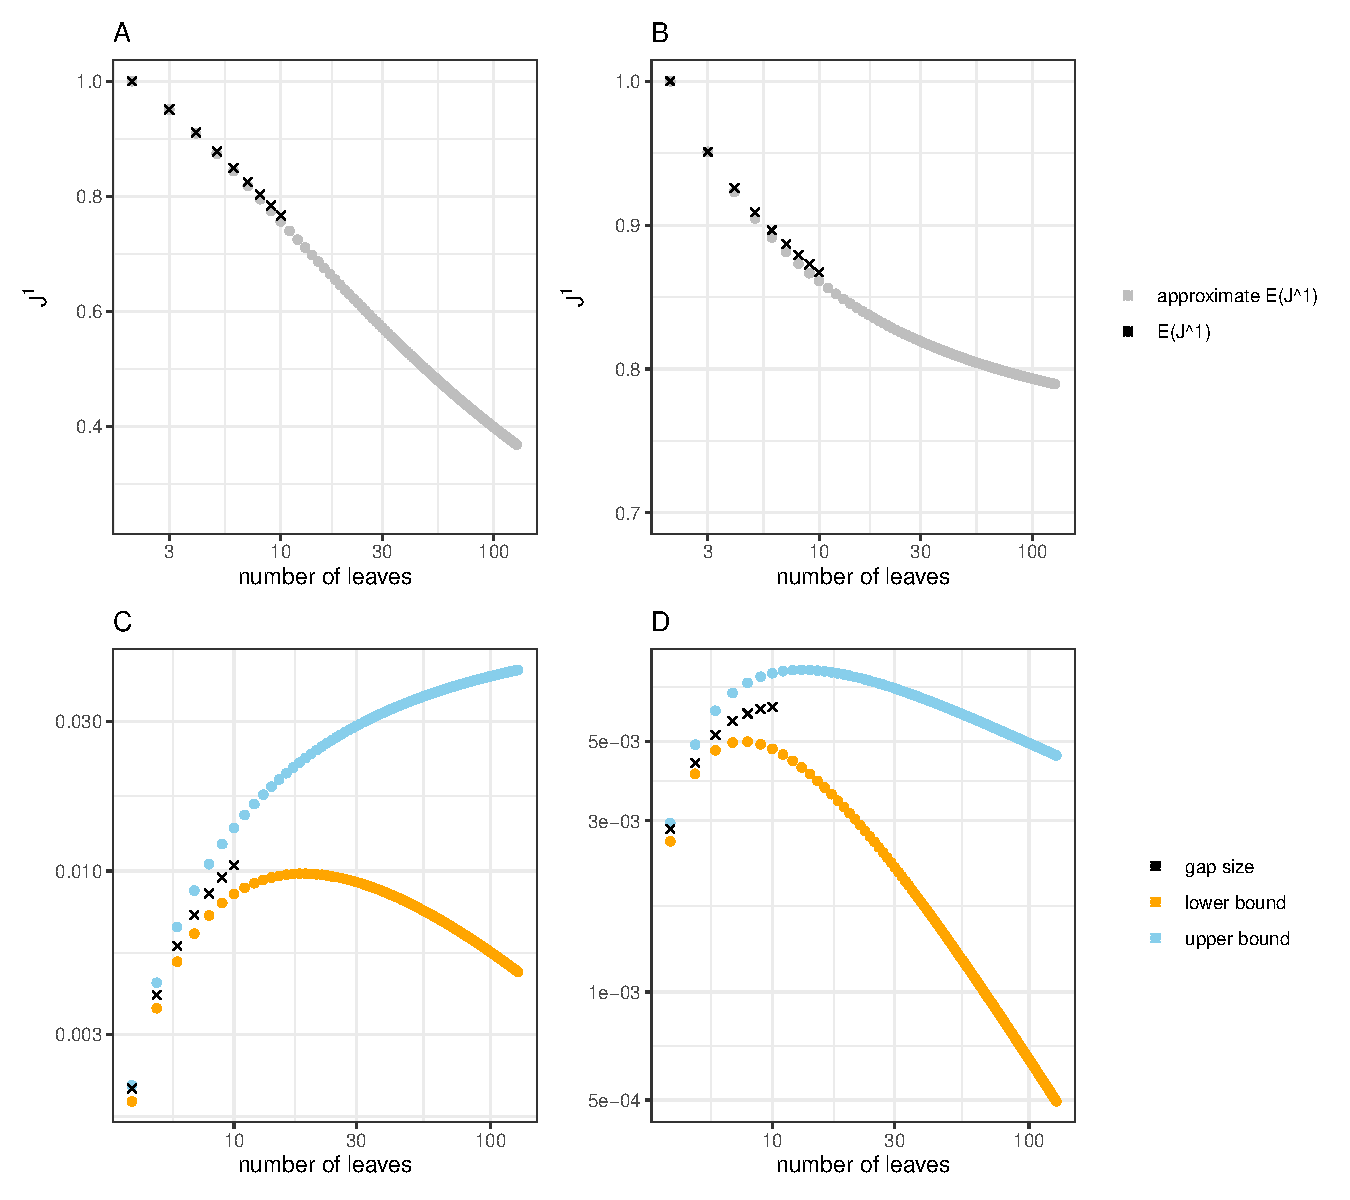
\includegraphics[width=\textwidth]{Chapter_trees/figures/jensenGapFigure.pdf}
    \caption{\textbf{Top row}: True values of $\mathbb E(J^1)$ for up to $10$ leaves were calculated manually, and the approximations up to $128$ leaves were calculated as $n\log_2n/\mathbb E(I_S)$. \textbf{A} --- uniform model, \textbf{B} --- Yule model.\\
    \textbf{Bottom row}: The Jensen gap of $\mathbb{E}(J^1)$ calculated for trees up to $128$ leaves under the uniform model (\textbf{C}), and the Yule model (\textbf{D}). The size of the gap is calculated as the difference between the true and approximate expected value, with the gaps for $2$ and $3$ leaves equal to zero as there is only one possible bifurcating tree shape for each of those values. Refer to tables \ref{table_yule} and \ref{table_unif} for numerical values of the gap size for the first several values of $n$.}
    \label{jensenfig} 
\end{figure}
In figure \ref{jensenfig}, we show behaviour of the Jensen gap and its bounds for $J^1$ under the Yule and uniform models.

Having a good approximation for the expected value of $J^1$ is a crucial result in the development of this index, as it allows us to employ it in the analysis of evolutionary processes on phylogenetic trees. The next step in this direction would be to obtain a closed-form solution for the expectation of $J^1$, as well as its variance.

\section{Analytic properties of the $J^1$ index}
A balance index is typically normalised by considering its extremal values for a given number of leaves \cite{fischer_tree_2021}. However, by its definition \cite{lemant_robust_2021}, $J^1$ follows a different normalisation procedure which in turn makes comparison of its values on trees of different sizes valid. The way $J^1$ was defined also makes it more complicated to define families of trees which maximise or minimise $J^1$ if we do not impose restrictions on the tree topology or node size distribution. In this section we do a bit of both, and consider only leafy trees with the out-degree of each internal node greater than $1$.

% look at the values of the edges of the relationship between the cophenetic index and J^1

	%\begin{itemize}
	%    \item a lot of this section is only relevant mathematically for completeness sake, rather than being applicable on real %data - especially the broom/caterpillar stuff
	%    \item \textbf{subsection} special trees - brooms, caterpillars, etc. present, discuss
	%    \item \textbf{subsection} tree ties - equivalence classes in index space, present, discuss
	%    \item \textbf{subsection} TBD
	%\end{itemize}
	
\subsection{Properties of $J^1$ on different tree families}
One may not encounter trees which yield extreme values of the balance index in practice often, if at all. However, it is still important to investigate the kinds of trees that maximise or minimise the index for the purposes of a complete mathematical discussion. 
	
\subsubsection{Some special tree topologies}
For most balance indices in use in evolutionary biology, the least balanced tree for a given number of leaves $n$ is the binary caterpillar tree. We have previously derived a general expression for leafy trees of this topology \cite{lemant_robust_2021}
\begin{equation}
    J^1(T_C) = \frac{2n\log_2n}{(n-1)(n+2)}.\label{caterpillar}
\end{equation}
Most balance indices in literature define the caterpillar topology as the least balanced one \cite{fischer_tree_2021}. Intuitively, this makes sense as balance is often associated with symmetry, and the caterpillar is the most asymmetric bifurcating tree. However, in the context of the $J^1$ index, tree topology is just one of a few factors which contribute to the balance score of a tree, especially since the index does not limit the space of trees to bifurcating ones. We also have to consider node sizes and, more specifically, how the population is split across different subtrees in the tree of interest. Let us consider a slightly altered caterpillar topology.
\par
\begin{figure}
    \centering
    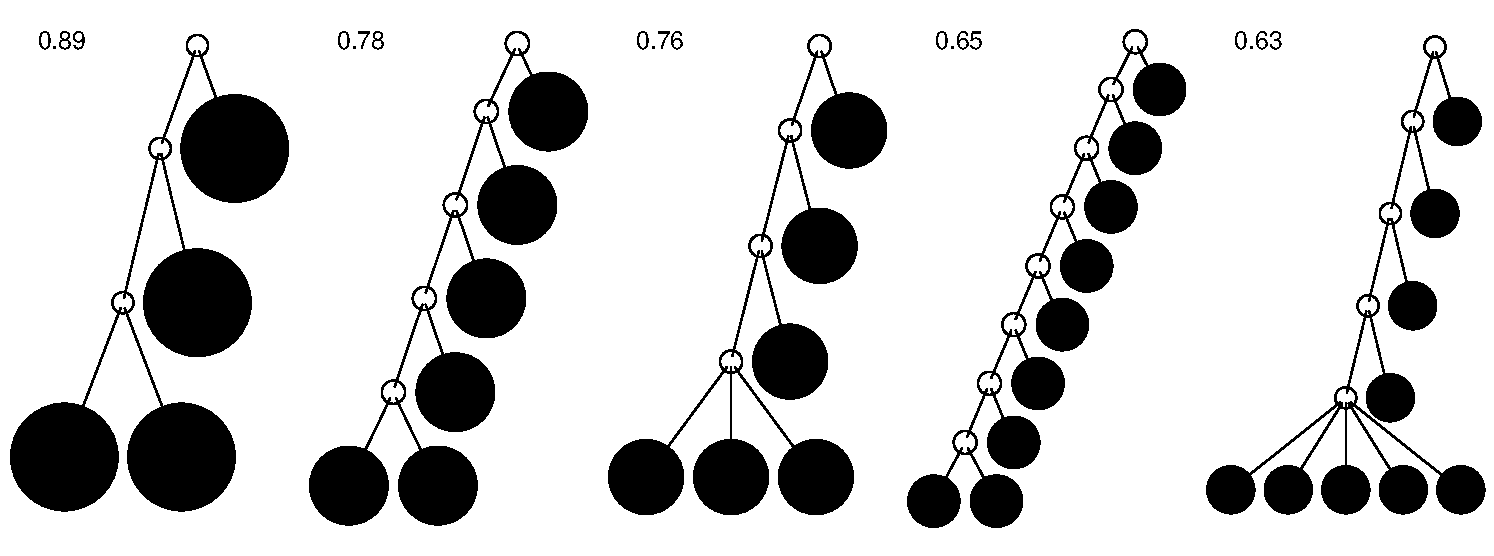
\includegraphics[width=\textwidth]{Chapter_trees/figures/example_figure_1.pdf}
    \caption{If we limit our search to leafy trees, the least balanced tree on a given number of leaves is not necessarily the caterpillar. Pictured are the caterpillar trees on $4$, $6$, and $9$ leaves, as well as minimally balanced brooms for $6$ and $9$ leaves, with corresponding $J^1$ values.}
    \label{example_figure_1}
\end{figure}

\begin{definition}
    Let $T_B$ be a leafy tree on $n$ leaves. Let every internal node of $T_B$ except for the one with the highest depth have out-degree $2$ such that one of its descendants is a leaf, and the other an internal node. Further, let the internal node most distant from the root have out-degree $k$. Then we call tree $T_B$ a \textbf{broom tree}.
\end{definition}

We can derive a general expression of $J^1$ for this family of trees.

\begin{proposition}\label{broom_prop}
    The value of $J^1$ for a broom tree $T_B$ on $n$ leaves, of which $k$ in the broom head is
    \begin{equation}
         J^1(T_B) = \frac{2}{(n+k)(n-k+1)}\left( n \log_2 n - k \log_2 k + k \right).\label{J1Tb}
    \end{equation}
\end{proposition}

We can also generalise the result of proposition \ref{broom_prop} slightly in the following way.

\begin{proposition}\label{q-broom-prop}
For a broom tree $T_{Bq}$ on $n$ leaves, of which $k$ in the broom head, such that the sizes of leaves in the head sum to $q$, $q\in \mathbb R$, and the leaves in the ``handle" all of equal size $1$, the value of $J^1$ is
    \begin{align*}
        J^1(T_{Bq}) = &\frac{1}{(n-k+1)(q+(n-k)/2)}\\
        &\times\left( q\log_k q-\sum_{i=1}^{k}l_i\log_k l_i+(q+n-k)\log_2(q+n-k) - q\log_2q \right),\numberthis\label{J1Tbq}
    \end{align*}
        where $l_1,\dots,l_k$ are the leaf sizes which add up to $q$.
\end{proposition}

In figure \ref{example_figure_1} we show that the caterpillar is not the minimally balanced leafy tree for a few tree sizes. To take it a step further, consider the following proposition. 

\begin{proposition}\label{cat_prop}
    For leafy trees on $n$ leaves and no linear parts, the caterpillar minimises $J^1$ iff $n<5$.
\end{proposition}
\begin{proof}
    Let $J^1_B(n,k)$ denote the value of $J^1$ on a broom tree with $n$ leaves, of which $k$ in the broom head. Then
    \begin{align}
        J^1_B(n,2) = & \frac{2n\log_2n}{(n+2)(n-1)}, \label{j1bn2}\\
        J^1_B(n,3) = & \frac{2}{(n+3)(n-2)}(n\log_2n - 3\log_2 3 + 3).\label{j1bn3}
    \end{align}
    Consider the case when $J^1_B(n,2) < J^1_B(n,3)$. Plugging in equations \eqref{j1bn2} and \eqref{j1bn3}, we can rearrange the inequality to find
    \begin{equation}
        8n\log_2n - 6(n^2+n-2)\log_2 3 + 6(n^2+n-2) > 0,
    \end{equation}
    which changes sign at $0, 0.667, 1$ and $4.168$. Setting the first derivative of this expression to zero 
    \begin{equation*}
        8\log_2n+\frac{8}{\log 2}-(12n+6)\log_2 3 + 12n + 6 = 0
    \end{equation*}
    we find solutions around $n=0.822$ and $n=2.888$, the latter of which signifies a local maximum. Therefore, as $n$ can only take positive integer values, valid solutions for which the caterpillar is less balanced than the broom with $3$ leaves in the broom head according to the index $J^1$ are $3$ and $4$, with the $k=3$ broom being less balanced otherwise.
\end{proof}

This proposition gives us a threshold for the number of leaves at which the caterpillar is not longer the minimally balanced tree for the given number of leaves, which sets $J^1$ apart from traditionally defined balance indices. This comes with the benefit of the new index's robustness to removal of small nodes, universality, and generality. However, we are yet to prove the following statement.

\begin{conjecture}\label{conj}
    For leafy trees on $n$ leaves and no linear parts, the tree that minimises $J^1$ belongs to the broom family.
\end{conjecture}

\subsubsection{Behaviour as $n\to\infty$}
    
    \begin{figure}[h!]
        \begin{center}
        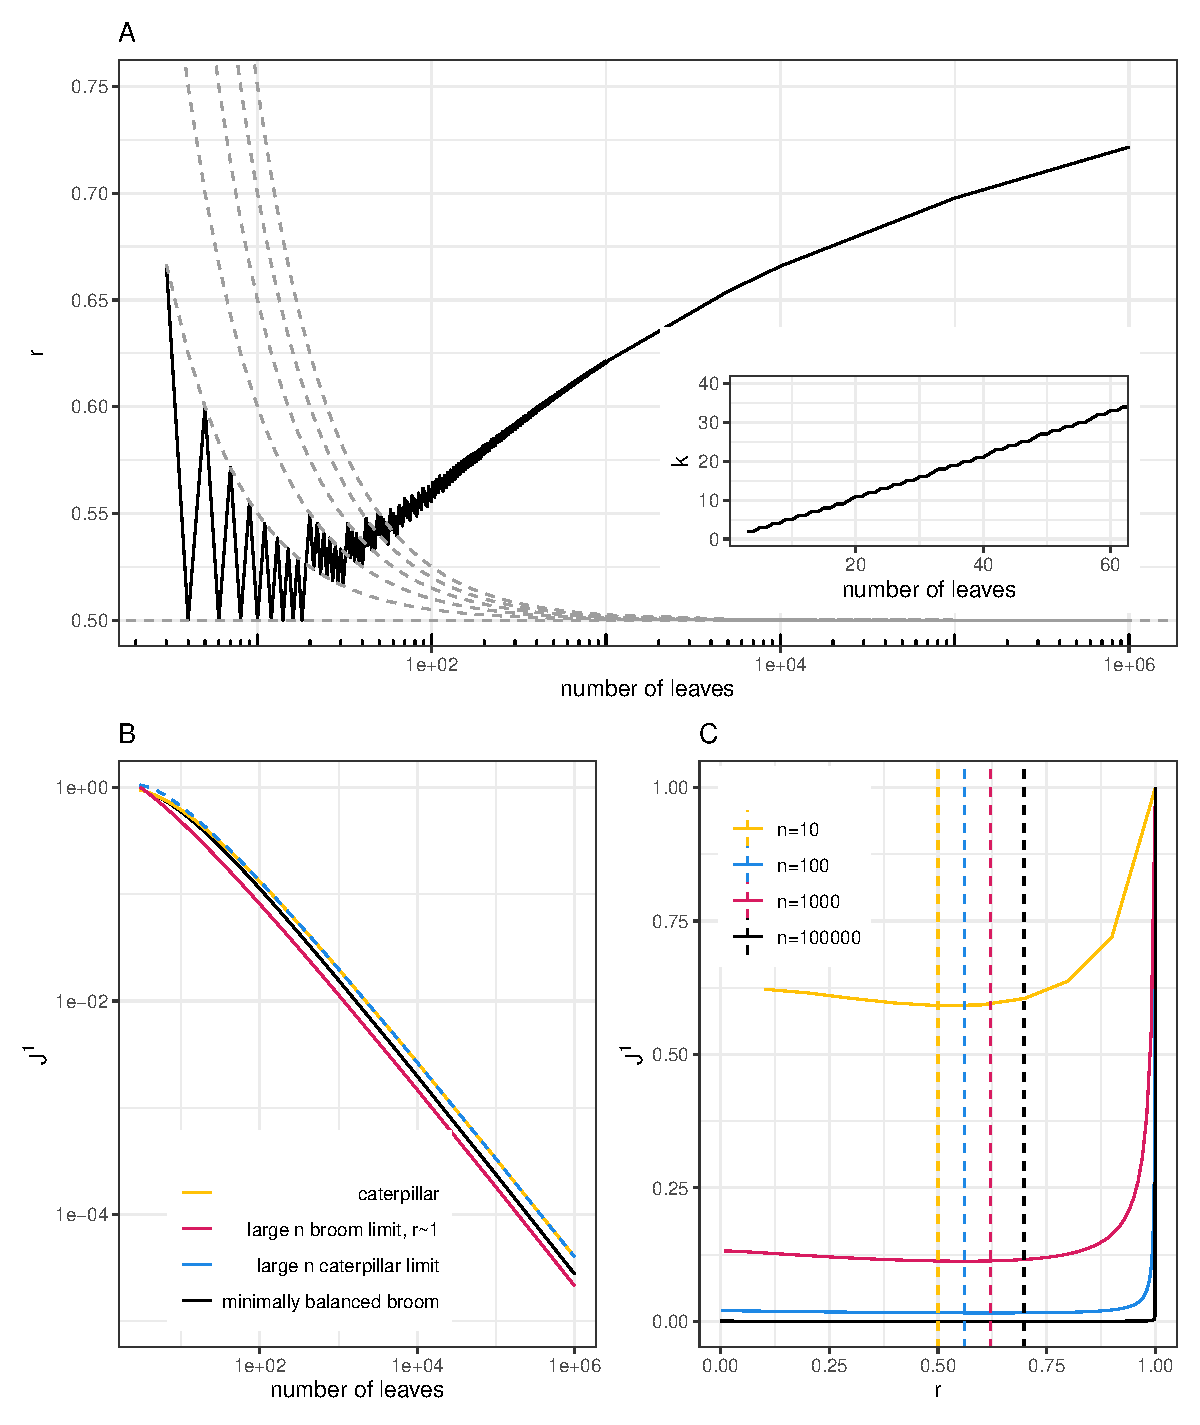
\includegraphics[width = \textwidth]{Chapter_trees/figures/figures_updated.pdf}
        \caption{The labels used in the figures are as above - $n$ for number of leaves, $k$ for number of leaves in the broom head, $r=n/k$. \textbf{A:} Value of $r$ for which the minimum value of $J^1$ is obtained on leafy trees. Trees on $n$ leaves which satisfy $r = \frac{n+a}{2n}$, for $a=0,1,2,\dots$ lie on the dashed grey lines. \textbf{B:} Behaviour of caterpillar and broom for different values of $n$. \textbf{C:} $J^1$ for different broom trees on a given number of leaves using equation \eqref{J1Tb}. The dashed lines indicate the value of $r$ for which $J^1$ is minimal.}
        \label{Rfigures}
        \end{center}
    \end{figure}

    % try and figure out a closed form expression for the bounds on n vs r - could help figure out what's going on in the formula
    %add m-ary caterpillar curves to the figure as well - relevant
We have derived general behaviour of $J^1$ on broom and caterpillar trees for a given number of leaves $n$. However, as some of the equations implied are not analytically solvable (e.g., conjecture \ref{conj}) we also explore asymptotic behaviour of $J^1$.
%find general expression for full m-ary caterpillar
%simplest case caterpillar is for bifurcating trees, now we extend to full m-ary trees
If we let $n\to\infty$, the value of $J^1$ for the caterpillar from equation \eqref{caterpillar} will behave like
    \begin{equation}
        \lim_{n\to\infty} J^1(T_C) = \frac{2\log_2n}{n}. \label{caterpillarlim}
\end{equation}

As $J^1$ is not limited to trees with equal leaf sizes, there is a threshold we can impose on the broom tree beyond which the caterpillar is less balanced.

\begin{proposition}\label{p-broom-prop}
    Let $T_B(n)$ be a broom tree on $n$ leaves such that the leaves on the handle and head have sizes $f$ and $fp$ respectively, and $T_C(n)$ be a caterpillar tree on $n$ leaves of equal sizes $f$. Then
    \begin{equation}\label{p-broom-cond}
        J^1(T_B) > J^1(T_C) \text{\quad iff \quad} p<\frac{1}{2},
    \end{equation}
    as $n\to\infty$.
\end{proposition}

For broom trees, the behaviour is a little more complicated and, perhaps, counterintuitive. Consider the following.
\begin{proposition}\label{ropt_prop}
    Let $\mathcal{T}_B(n)$ be the set of all broom trees on $n$ leaves, $r = \frac{k}{n}$ where $k$ is the number of leaves in the broom head for a given tree, and $r_\text{opt}$ the value of $r$ which minimises $J^1$ for a given $n$. Then $r_\text{opt}\to 1$ as $n\to\infty$.
\end{proposition}
The proposition says that most leaves on a minimally balanced broom tree will be concentrated in the head, with comparatively few on the handle, resembling a start tree more closely than a caterpillar tree. However, one must take into account how imbalanced the nodes above the broom head are, since one of their subtrees contains most of the tree's leaves, whereas the other is a single leaf. 

\par 

Finding the true value of $k$ which minimises $J^1(T_B)$ analytically is difficult. The derivative with respect to $k$ of equation \eqref{J1Tb} yields a transcendental equation which is not analytically solvable.
    
\section{Discussion}
        %\begin{itemize}
         %   \item $J^1$ is not a traditional balance index, contains more information, more widely applicable
	%	\item while more general/universal than other indices, $J^1$ does not account for all information one might wish to include in a tree --- branch length discussion?
	%\end{itemize}

The main aim of this paper was to explore deeper analytic properties of the robust, universal balance index $J^1$ and start finding its place in the broader context of tree balance by extending past results and uncovering new connections. \par
There are still areas where the index $J^1$ falls short in terms of generality. The balance of a tree whose branch lengths differ is not a case that the new index can handle. This opens up the possibility of further generalisation of the index and future research.\par
Finally, we only touched upon directly obtainable relationships without considering different real-world use cases of the index and the implications of equation \eqref{prop6}. This is another avenue of future research as there may exist a relationship between the way indices vary with time and the underlying evolutionary process growing the associated tree.


\chapter{Tracking cancer evolution \textit{in silico} via evolutionary indices}
\textit{Part of the results from this chapter were presented in poster form at MMEE 2022 in Reading and at ECMTB 2022 in Heidelberg.}

\begin{itemize}
    \item \textit{summarising the properties of trees is very useful}
    \item \textit{how many indices are enough to distinguish them?}
    \item \textit{check figure 8 in Rob's new preprint}
\end{itemize}

\section{Introduction}
A trajectory is a path described by any object (or indeed point) in some space according to some parameter, usually time.  Intuitively then, an evolutionary trajectory refers to the path or sequence of changes and adaptations that a lineage or population undergoes over time. It describes the series of genetic, morphological, and behavioral transformations that occur as organisms evolve and diversify. We are interested in the evolutionary trajectory of cancers but obtaining reliable data over time is not feasible in reality. This stems from multiple issues. Firstly, at time of diagnosis, solid tumours have likely already been growing for long enough to reach a size visible in standard medical imaging (citation needed). This means that even initial data obtained in the clinic represents a relatively late stage in the cancer's evolutionary history. Secondly, solid tumours are clumps of cells organised in some way in space, meaning that taking a sample from one point in the tumour is not necessarily representative of the rest of the cell population. Finally, a biopsy is an invasive procedure which can cause considerable discomfort to patients, depending on where the tumour is situated. Therefore, having a reasonable estimate of a tumours evolutionary trajectory based on the data that is available at time of sequencing would be extremely useful.

\subsection{Why even bother with indices?}
Before we begin, let us consider the simplest question - can we map the set of all possible trees to the set of real numbers? For this purpose we should decide how to define the set of trees. The number of nodes in a tree is a natural number, $n\in\mathbb{N}$, as is the number of possible tree topologies for a given $n$. We denote with $T(n)$ the set of enumerated tree topologies (cite Nakano). Each node then has a corresponding size, giving as an $n$-tuple of real numbers $(\alpha_1, \dots, \alpha_n)\in\mathbb{R}^n$, and each edge (branch) has a corresponding length or $(l_i, \dots, l_{(n-1)})\in\mathbb{R}^{(n-1)}$. This means we would need a family of maps 
\begin{equation}
    f_n: A(n) \times \mathbb{R}^n \times \mathbb{R}^{n-1} \rightarrow R.
\end{equation}
We can thus easily assign real values to distinct trees. The only problem with this approach is that it is not at all useful, not least due to its lack of any interpretability. This chapter outlines an approach which uses real-valued summaries of trees' properties in a way that is both intuitive and mathematically robust. 

\section{Picking a tree out of a line-up}
\begin{itemize}
    \item using numerical summaries may sound reasonable, but does it produce distinct enough results?
    \item what is the minimal number of indices we need to consider to tell apart two trees in general
    \item how about in the context of realistic data (e.g. driver trees)?
\end{itemize}
To show that there is merit to the idea of constructing evolutionary trajectories in an index space, let us consider the case where distinct trees have equal values of all indices in our desired set. 
\subsection{Examples of distinct trees with identical index values}
\begin{itemize}
    \item we begin by examining the simplest case - leafy trees with equal leaf sizes
    \item consider first the smaller set of indices ($J^1$, $D_{Shannon}$, $N_{drivers}$)
    \item in this case we can construct a family of trees based on the canonical factorisation of $n$, the number of leaves
    \item then show what this looks like on the expanded set of indices (Rob \& Kim)
    \item all of these trees are perfectly balanced and symmetric, making them an unlikely appearance in real data (cite data papers to show what real data looks like, e.g. TracerX)
    \item loosening up our criteria for what a tree looks like we consider leafy trees with arbitrary node sizes
    \item can again construct artificial examples for the smaller set of indices
    \item more difficult for the expanded set
\end{itemize}

\section{Computational methods}
\subsection{Agent-based modelling framework - \textit{warlock/demon}}
There is no shortage of agent-based models of tumour evolution (cite Blair's review), and the can range from purpose-built complex frameworks to more stripped-down and abstract ones. Since each model should be ``as simple as possible but no simpler", the appropriate framework for our purposes must satisfy certain requirements --- flexibility, efficiency, and reproducibility. The first requirement is deceptively specific. As the main inspiration behind this work stems from cancer evolution, we want our simulations to have parameters for controlling aspects of the cell population's physical properties which would in turn imply a different way in which it evolves. This would, for example, include spatial arrangement of cells, mutation rates, migration rates, and selective advantage. Furthermore, while the goal is to simulate large populations of cells, we also need a large number of simulations over which we can infer more general deterministic properties. Stochastic effects could make vastly different evolutionary modes look more similar than expected in theory. Finally, reproducibility allows us to share parameters of our models for verification by peers, and possible further investigation.\\
The agent-based modelling framework we decided to use is \texttt{warlock} (cite warlock preprint), a \texttt{snakemake} (cite snakemake paper) wrapper written for \texttt{demon} (cite demon repo). It satisfies the requirements above, with a few associated comments. Firstly, it is a flexible agent-based model of tumour evolution as it does have parameters which control for spatial arrangement, mutation rates and selective advantage, as well as migration. While it is able to simulate spatial structure, \texttt{demon} covers at most two spatial dimensions. This is not an issue since we approximate the cell population to undergo stochastic isotropic growth, that is the tumour has equal probability of expanding in all directions in space. This implies approximate spherical symmetry of simulated solid tumours, which allows us to effectively consider the two-dimensional simulation as a cross-section of a tumour spheroid. In terms of efficiency, \texttt{demon} was written mainly in C++, and conceptualised so that instead of tracking individual cells, it simulates unique cell genotypes on a two-dimensional grid comprised of demes, or well-mixed patches of cells. The procedure for simulation cell events is based on the Gillespie algorithm (cite Gillespie), and follows the steps of selecting a deme, then cell type, event type, and finally cell genotype. This approach sacrifices micro-scale interactions between cells to benefit efficiency and the feasibility of mathematical analysis of the model using, for example, diffusion approximations. Finally, all associated code is free and open source (cite github repos), which allows reproducibility using identical parameters and random seeds. Parameter values for different batches can be found in the appendix (ref).

\subsection{Smaller set of tree indices}
\begin{itemize}
    \item $J^1$ balance index
    \item mean number of drivers per cell
    \item Shannon diversity
    \item mean node out-degree
\end{itemize}

\subsection{Expanded set of tree indices}
\begin{itemize}
    \item explain the work behind Rob and Kim's paper
    \item reference the paper and repo with the code for calculating the indices
\end{itemize}

\section{Results}
\subsection{Spatial constraints influence index space trajectories}
\begin{itemize}
    \item figure of trajectories and the average trajectory for each spatial mode (both smaller and expanded index set)
    \item figures should be arranged on a grid dependant on parameter values
    \item compare to Rob's modes of evolution paper in both instances (base index set and expanded) and discuss
\end{itemize}
\subsection{Late-stage index-space location implies mode of evolution (?)}
\begin{itemize}
    \item focus on the overlaps between (average and overall) trajectories of different processes at later stages of tumour growth
    \item consider differences between the base and expanded set of tree indices
    \item based on outputs, come up with a summary statistic which could sort a tumour into different based on the end-of-growth state of the tree
\end{itemize}

\section{Discussion}

\chapter{Agent-based workflow for inferring evolutionary parameters from molecular data using approximate Bayesian computation}\label{demonchap}
In this chapter, I will go over the methods I have used and developed for work on data in chapter \ref{methchap}. 

\section{Introduction}
\subsection{Spatial agent-based modelling}
\begin{itemize}
    \item go over a few relevant models in the field and how they compare to demon
    \item discuss the general assumptions and limitations of ABM
\end{itemize}


\subsection{Approximate Bayesian computation (ABC)}
\begin{itemize}
    \item high-level introduction of ABC
    \item papers in the field which have used some form of ABC
\end{itemize}

\section{Initial simulation workflows}
\begin{itemize}
    \item go over the old \texttt{demon} simulations with \texttt{demonmeth} R package analysis
    \item discuss why the approach worked
    \item point out the ways in which it didn't exactly work (i.e. impossible to get independent methylation and demethylation rates; output files sometimes too large to import into R and analyse efficiently; sometimes large files may not contain all the required data)
\end{itemize}

\section{Simulating fluctuating methylation arrays with \texttt{methdemon}}
\subsection{Overview}
\begin{itemize}
    \item go over the simulation's inner workings
    \item provide estimates of running efficiency and memory requirements
    \item discuss possible upgrades and their potential computational costs
\end{itemize}
\subsection{Examples}
Provide example outputs (and their visualisations), parameter tables and a citation/link to the github repo.

\section{Fluctuating methylation arrays through the lens of ABC}
\subsection{Overview}
\begin{itemize}
    \item go over the \texttt{pyabc} package briefly (cite)
    \item explain the ABC workflow
    \item discuss computational costs and efficiency
    \item discuss whether this is the best approach (can we write down a likelihood for the problem?)
\end{itemize}
\subsection{Examples}
Provide example applications of the workflow to \texttt{methdemon} outputs - fit smaller simulations to a big one for example.

\chapter{Inferring evolutionary parameters of colorectal cancer from DNA methylation arrays}\label{methchap} % consider splitting into a methods and data chapter - first one describing the modelling approach and is simulation-based, the second one expanding onto the real data
\chapter{Discussion}

%Appendices
\appendix
\chapter{Trajectories}\label{app:trajs}

\begin{table}[h]
\centering
\begin{tabularx}{0.75\textwidth}{|X|X|}
\hline
Parameter & Values \\
\hline
    Deme carrying capacity & $1, 512, 8192, \infty$ \\
    Driver mutation rate & $10^{-6}, 10^{-5}, 10^{-4}$ \\
    Selection coefficient & $0.05, 0.1, 0.2$ \\
    Baseline death rate (non-spatial) & $0.98$ \\
    Baseline death rate (spatial) & $0$ \\
\hline
\end{tabularx}
\caption{Parameters used for the simulations. The deme carrying capacity is
    varied across spatial configurations (boundary growth, invasive glandular,
    gland fission, non-spatial respectively), while other parameter variations
    are common to all simulations.}
\label{tab:traj_params}
\end{table}

\begin{figure}[h]
\centering
\includegraphics[width=\textwidth]{Chapter_3/figures/gland_time.png}
\caption{All trajectories in time for the new set of indices plotted for gland
    fission with the average trajectories for different sets of indices plotted
    in colour.}
\label{fig:gland_time}
\end{figure}

\begin{figure}[h]
\centering
\includegraphics[width=\textwidth]{Chapter_3/figures/inv-gland_time.png}
\caption{All trajectories in time for the new set of indices plotted for
    invasive glandular evolution with the average trajectories for different
    sets of indices plotted in colour.}
\label{fig:inv-gland_time}
\end{figure}

\begin{figure}[h]
\centering
\includegraphics[width=\textwidth]{Chapter_3/figures/boundary_time.png}
\caption{All trajectories in time for the new set of indices plotted for
    boundary growth with the average trajectories for different
    sets of indices plotted in colour.}
\label{fig:boundary_time}
\end{figure}

\begin{figure}[h]
\centering
\includegraphics[width=\textwidth]{Chapter_3/figures/non-spatial_time.png}
\caption{All trajectories in time for the new set of indices plotted for
    non-spatial tumours with the average trajectories for different
    sets of indices plotted in colour.}
\label{fig:non-spatial_time}
\end{figure}

\begin{figure}[h]
\centering
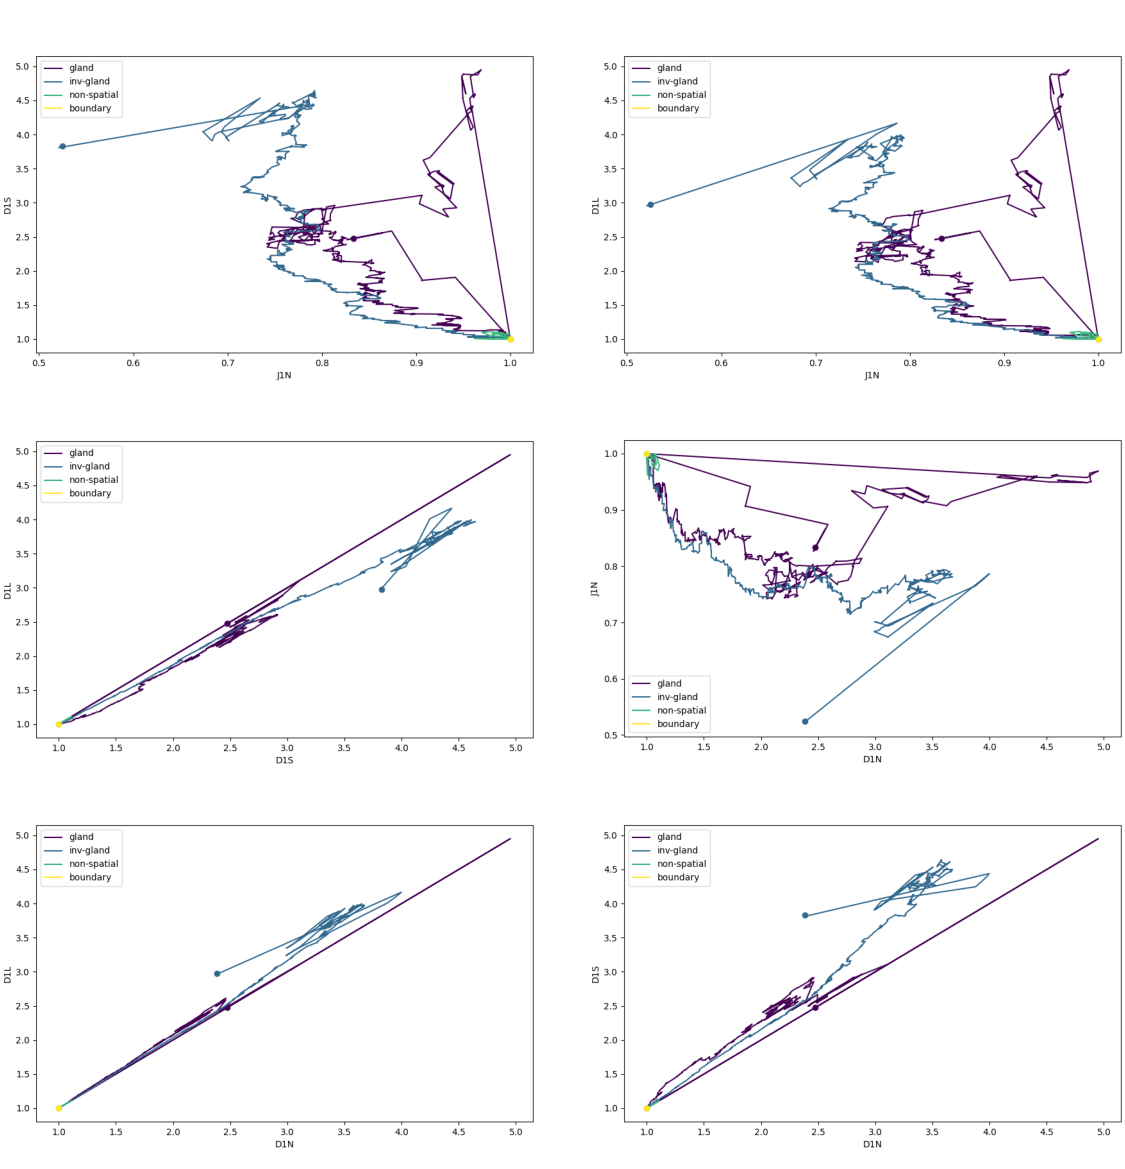
\includegraphics[width=\textwidth]{Chapter_3/figures/1e06005new.pdf}
\caption{Trajectories plotted for the four different spatial configurations for
    the driver mutation rate $\mu=10^{-6}$, and selective coefficient
    $s=0.05$.}
\label{fig:1e06005new}
\end{figure}

\begin{figure}[h]
\centering
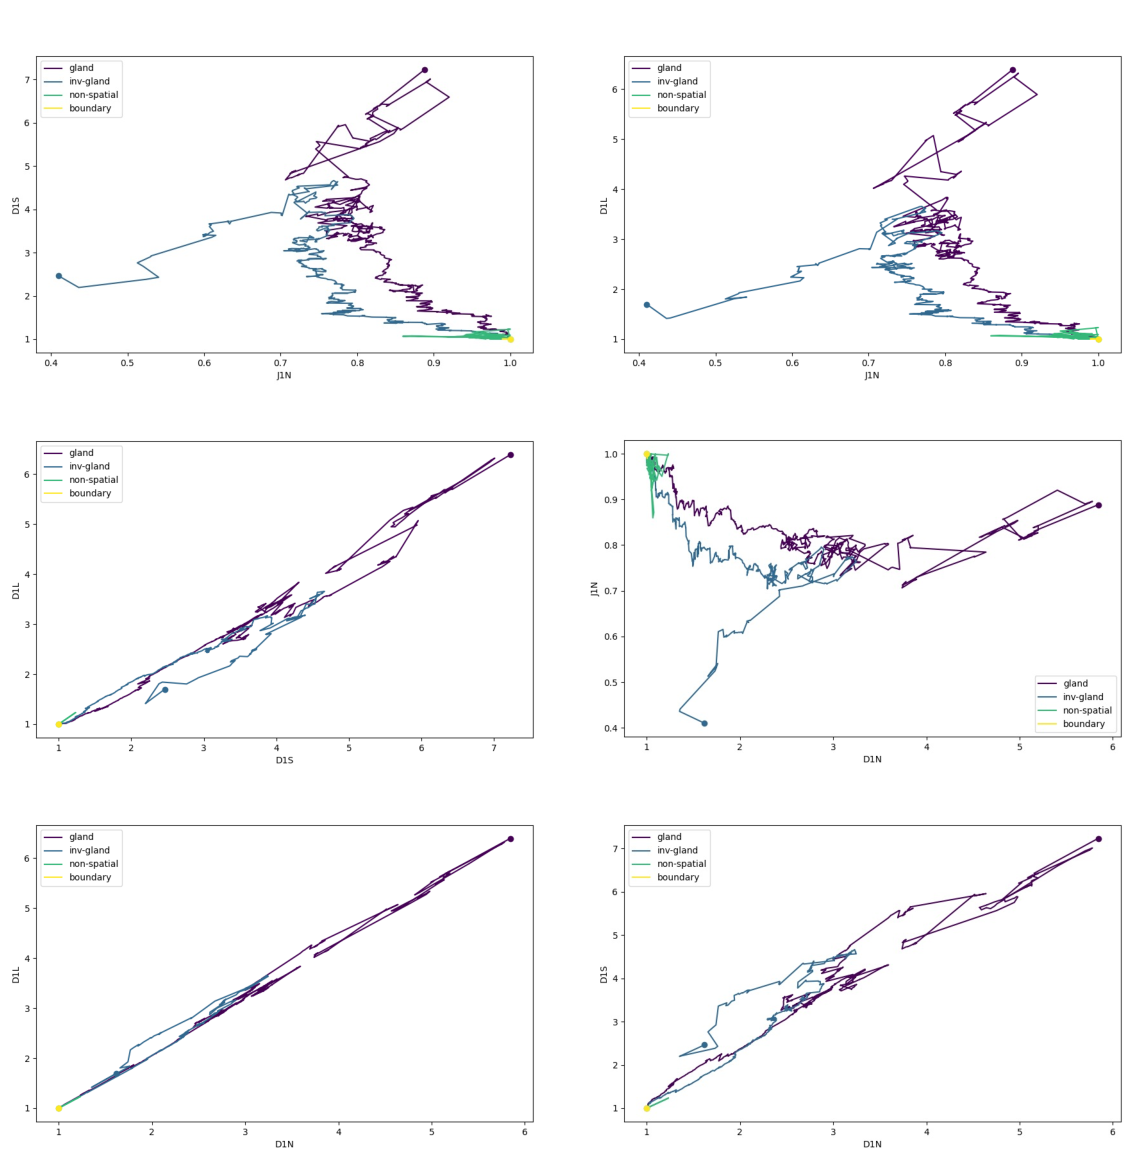
\includegraphics[width=\textwidth]{Chapter_3/figures/1e0601new.pdf}
\caption{Trajectories plotted for the four different spatial configurations for
    the driver mutation rate $\mu=10^{-6}$, and selective coefficient
    $s=0.1$.}
\label{fig:1e0601new}
\end{figure}

\begin{figure}[h]
\centering
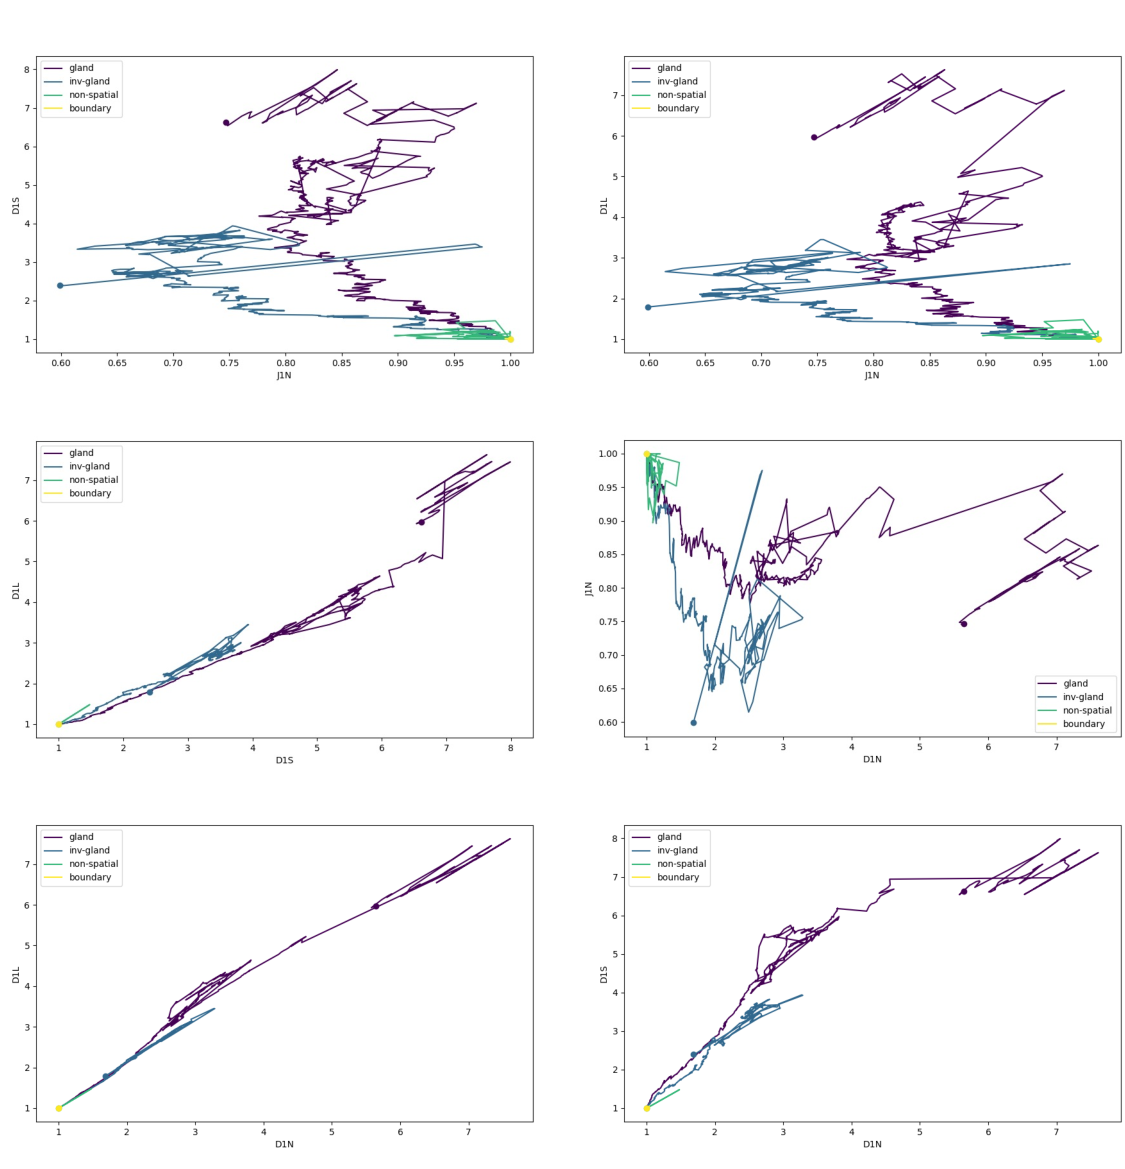
\includegraphics[width=\textwidth]{Chapter_3/figures/1e0602new.pdf}
\caption{Trajectories plotted for the four different spatial configurations for
    the driver mutation rate $\mu=10^{-6}$, and selective coefficient
    $s=0.2$.}
\label{fig:1e0602new}
\end{figure}

\begin{figure}[h]
\centering
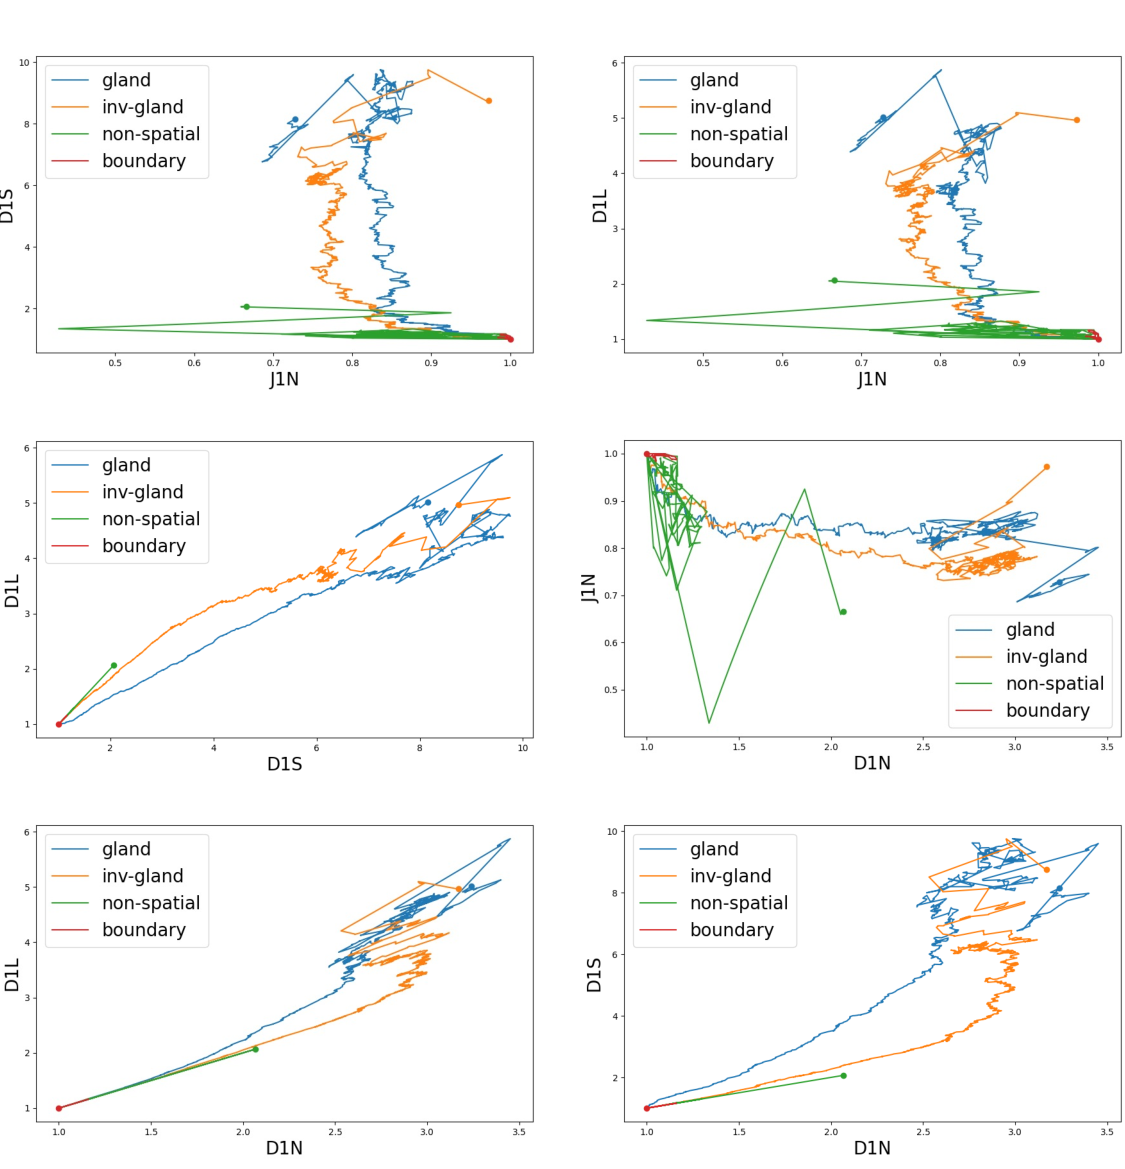
\includegraphics[width=\textwidth]{Chapter_3/figures/1e05005new.pdf}
\caption{Trajectories plotted for the four different spatial configurations for
    the driver mutation rate $\mu=10^{-5}$, and selective coefficient
    $s=0.05$.}
\label{fig:1e05005new}
\end{figure}

\begin{figure}[h]
\centering
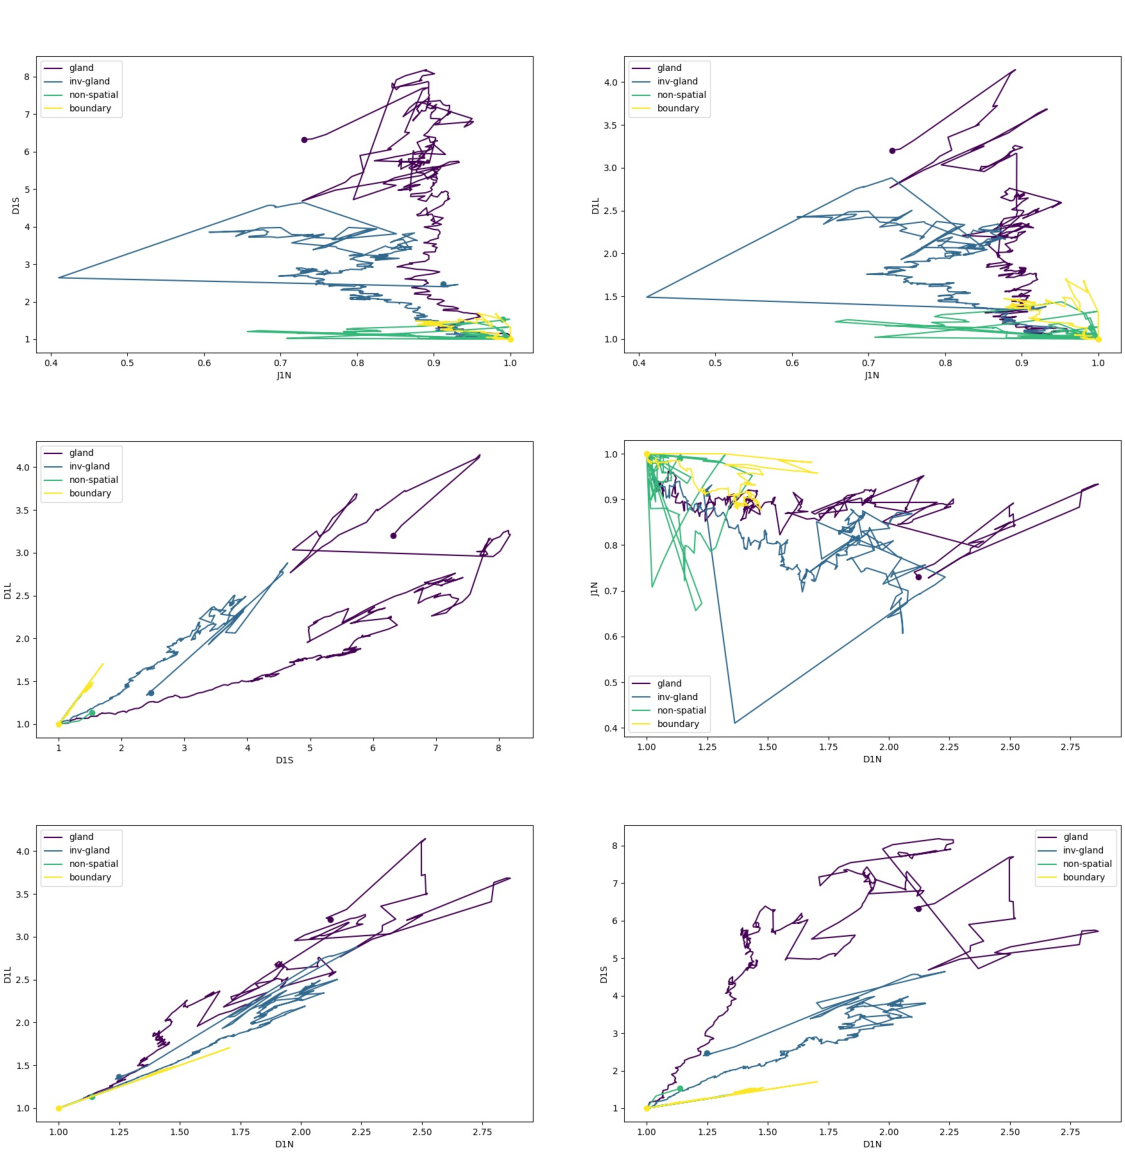
\includegraphics[width=\textwidth]{Chapter_3/figures/1e0502new.pdf}
\caption{Trajectories plotted for the four different spatial configurations for
    the driver mutation rate $\mu=10^{-5}$, and selective coefficient
    $s=0.2$.}
\label{fig:1e0502new}
\end{figure}

\begin{figure}[h]
\centering
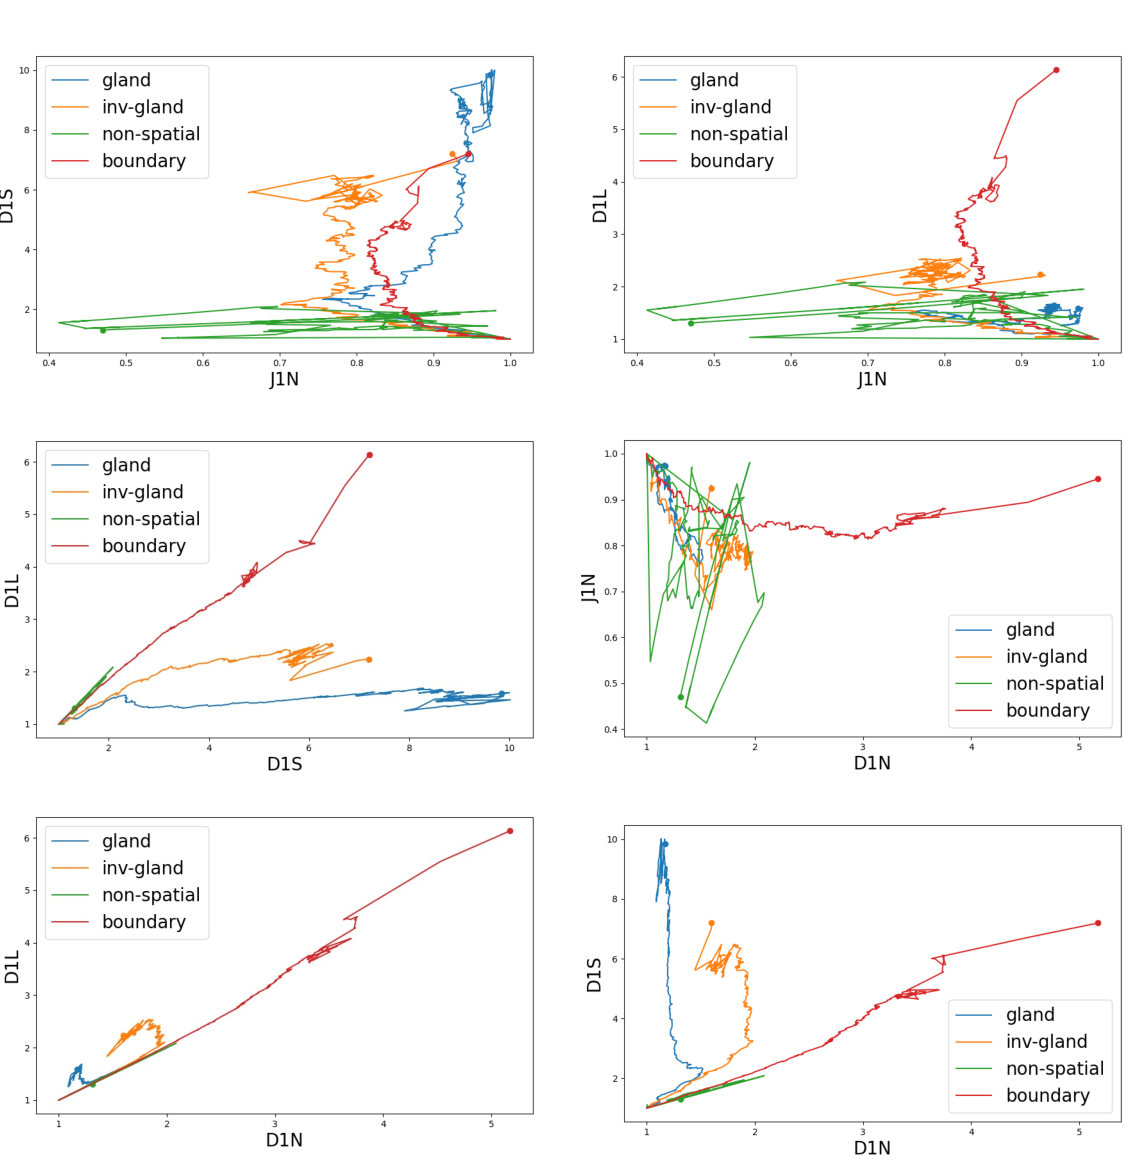
\includegraphics[width=\textwidth]{Chapter_3/figures/1e0401new.pdf}
\caption{Trajectories plotted for the four different spatial configurations for
    the driver mutation rate $\mu=10^{-4}$, and selective coefficient
    $s=0.1$.}
\label{fig:1e0401new}
\end{figure}

\begin{figure}[h]
\centering
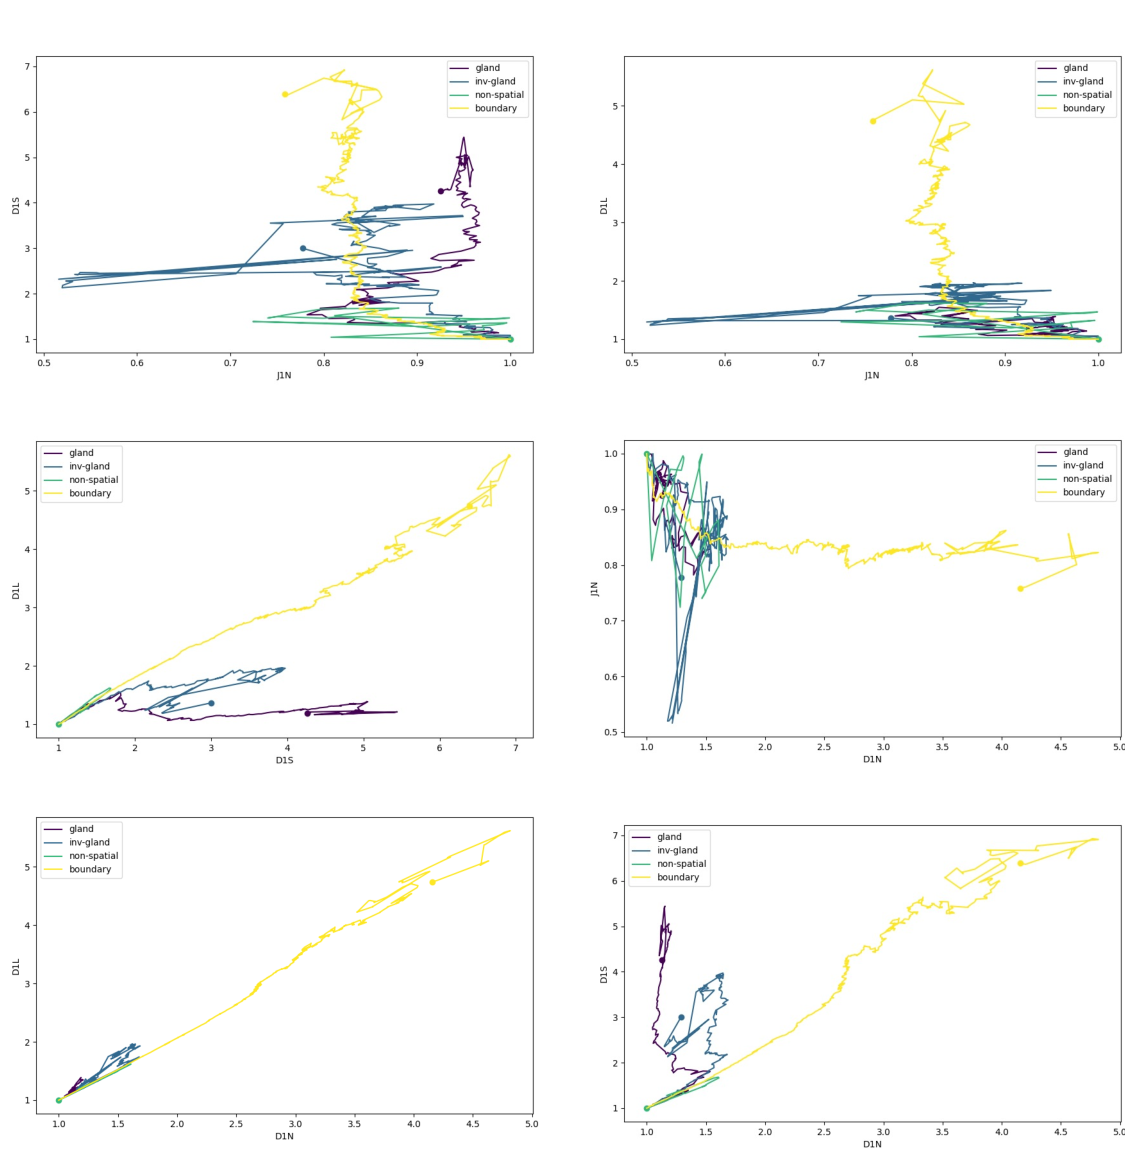
\includegraphics[width=\textwidth]{Chapter_3/figures/1e0402new.pdf}
\caption{Trajectories plotted for the four different spatial configurations for
    the driver mutation rate $\mu=10^{-4}$, and selective coefficient
    $s=0.2$.}
\label{fig:1e0402new}
\end{figure}

\begin{figure}[h!]
    \centering
    \includegraphics[width=\textwidth]{Chapter_3/figures/new_trajs2.png}
    \caption{Individual replicates' index trajectories of boundary growth for
    the parameters used in figure \ref{fig:1e05_01new}. }
    \label{fig:new_trajs2}
\end{figure}

\begin{figure}[h!]
    \centering
    \includegraphics[width=\textwidth]{Chapter_3/figures/new_trajs3.png}
    \caption{Individual replicates' index trajectories of gland fission for the
    parameters used in figure \ref{fig:1e05_01new}. }
    \label{fig:new_trajs3}
\end{figure}

\begin{figure}[h!]
    \centering
    \includegraphics[width=\textwidth]{Chapter_3/figures/new_trajs4.png}
    \caption{Individual replicates' index trajectories of non-spatial growth
    for the parameters used in figure \ref{fig:1e05_01new}. }
    \label{fig:new_trajs4}
\end{figure}





%% Back matter ------------------------------
\backmatter

%Appendices
\chapter{Parameter inference}\label{app:inference}

\begin{table}[h]
\centering
    \begin{tabularx}{0.85\textwidth}{|X|X|X|}
\hline
    Tumour & Median methylation rate & Median demethylation rate \\
\hline
    E & 0.0021 & 0.002  \\
    I & 0.005  & 0.0009 \\
    J & 0.0012 & 0.0018 \\
    S & 0.001  & 0.0033 \\
    X & 0.0008 & 0.0025 \\
\hline
\label{tab:inferred_epimutation_rates}
\end{tabularx}
\caption{Inferred epimutation rates for the tumour samples modelled in this
    thesis.}
\end{table}

\begin{figure}[ht]
\centering
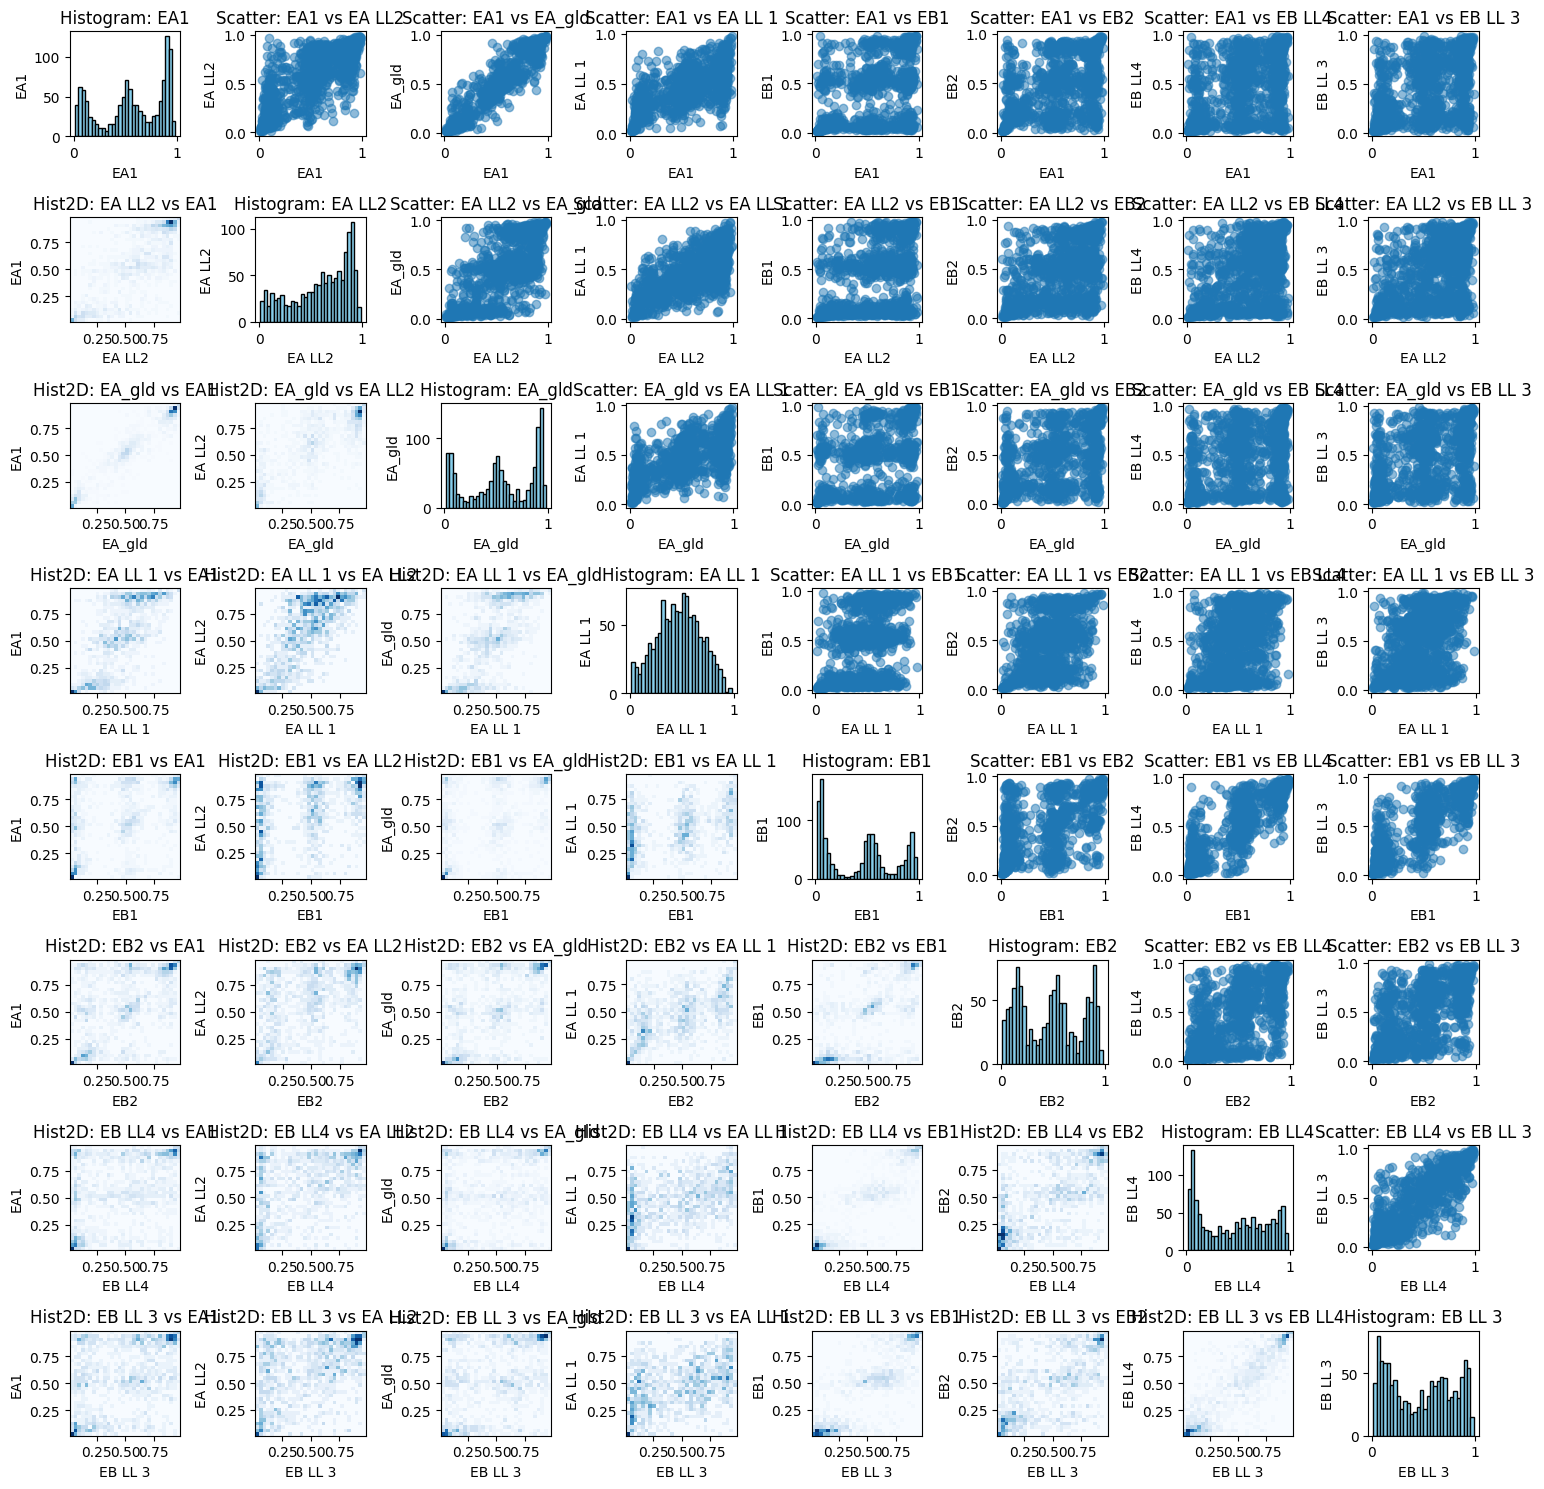
\includegraphics[width=\textwidth]{Chapter_5/figures/fCpG_loci_E.png}
\caption{Visualisation of fCpG arrays for patient E and the inter-gland
    correlation plots.}
\label{fig:vis_E}
\end{figure}

\begin{figure}[ht]
\centering
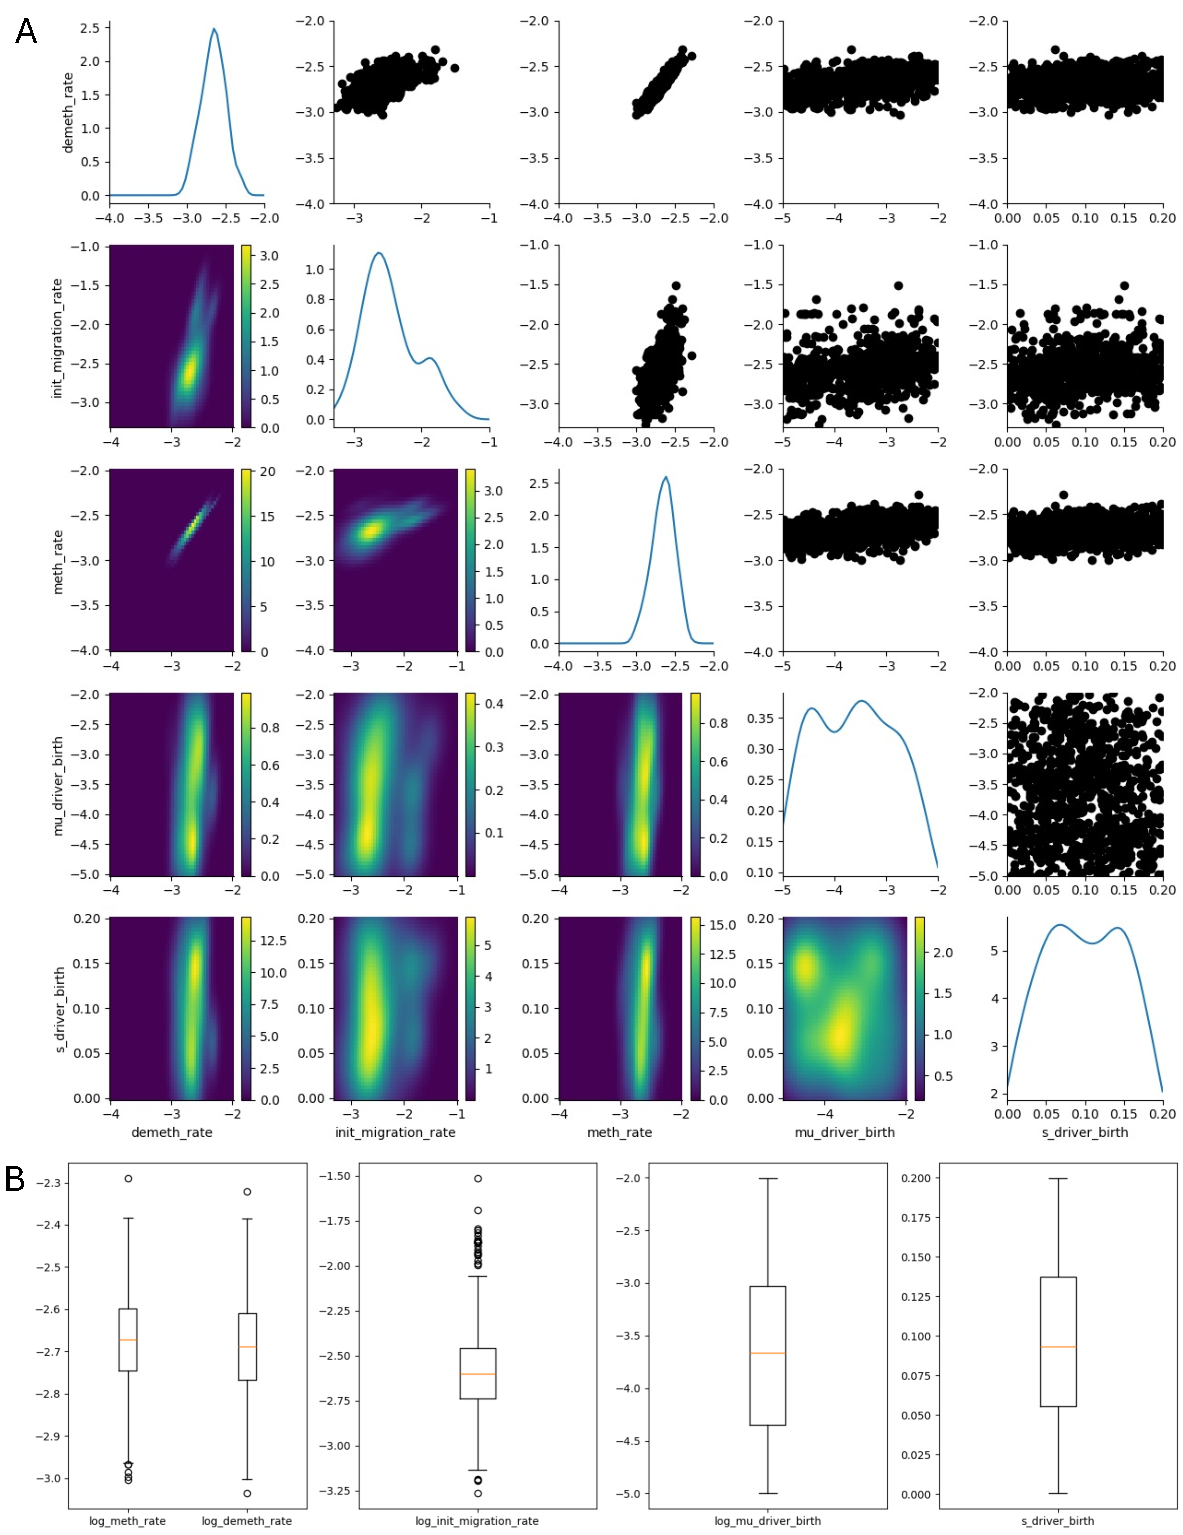
\includegraphics[width=\textwidth]{Chapter_5/figures/inference_E.pdf}
\caption{Parameter inference plots for patient E.}
\label{fig:inference_E}
\end{figure}

\begin{figure}[ht]
\centering
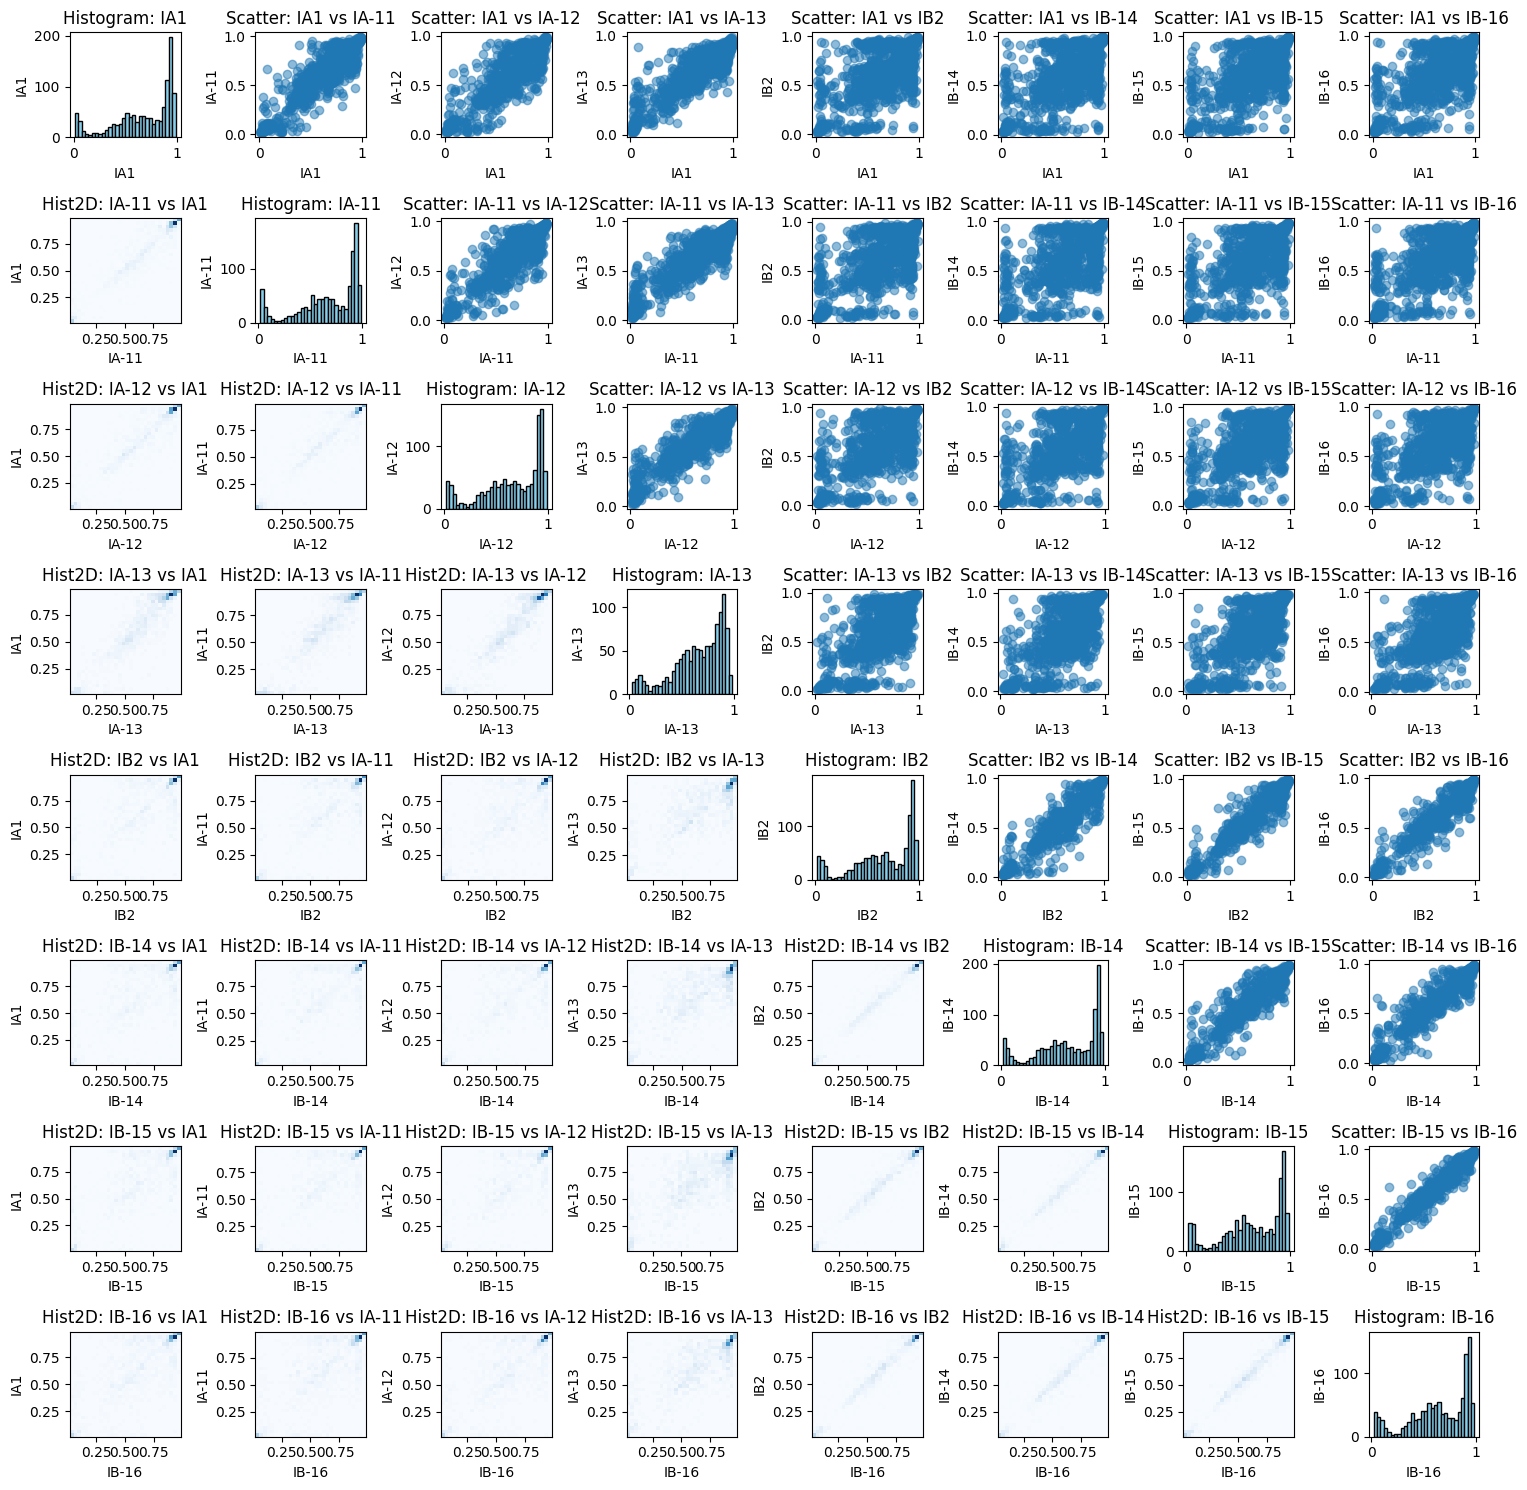
\includegraphics[width=\textwidth]{Chapter_5/figures/fCpG_loci_I.png}
\caption{Visualisation of fCpG arrays for patient I and the inter-gland
    correlation plots.}
\label{fig:vis_I}
\end{figure}

\begin{figure}[h]
\centering
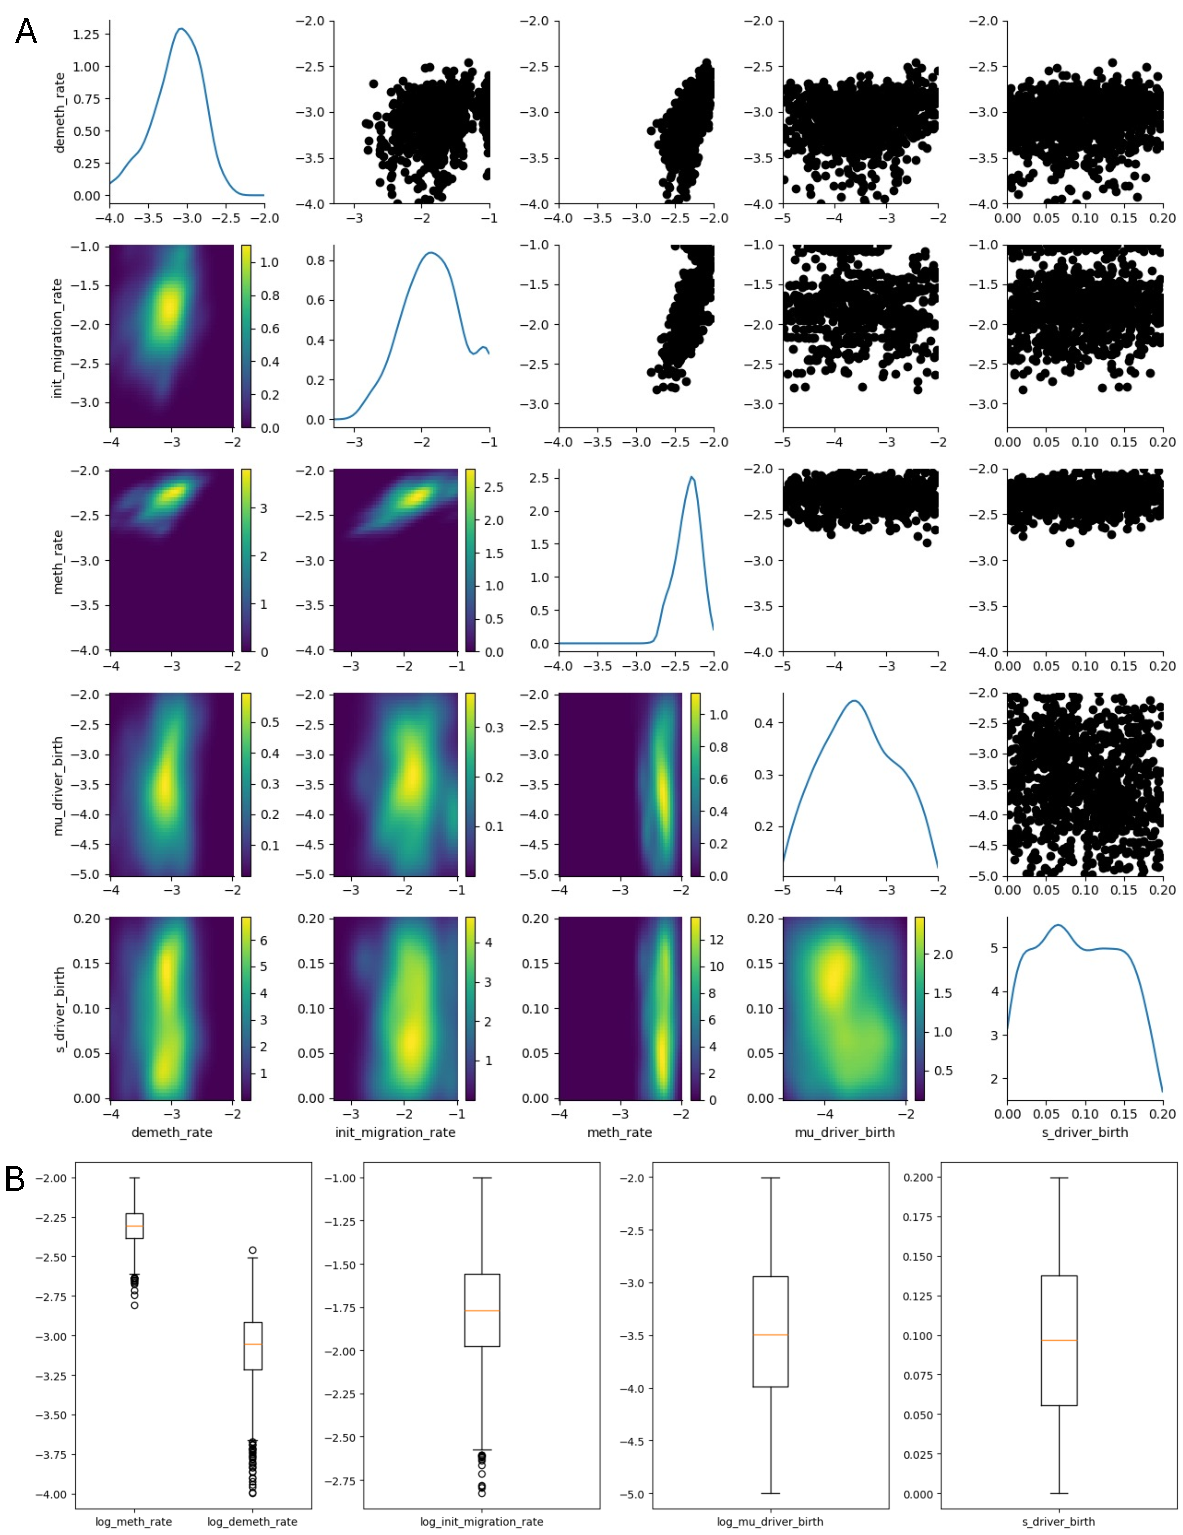
\includegraphics[width=\textwidth]{Chapter_5/figures/inference_I.pdf}
\caption{Parameter inference plots for patient I.}
\label{fig:inference_I}
\end{figure}

\begin{figure}[ht]
\centering
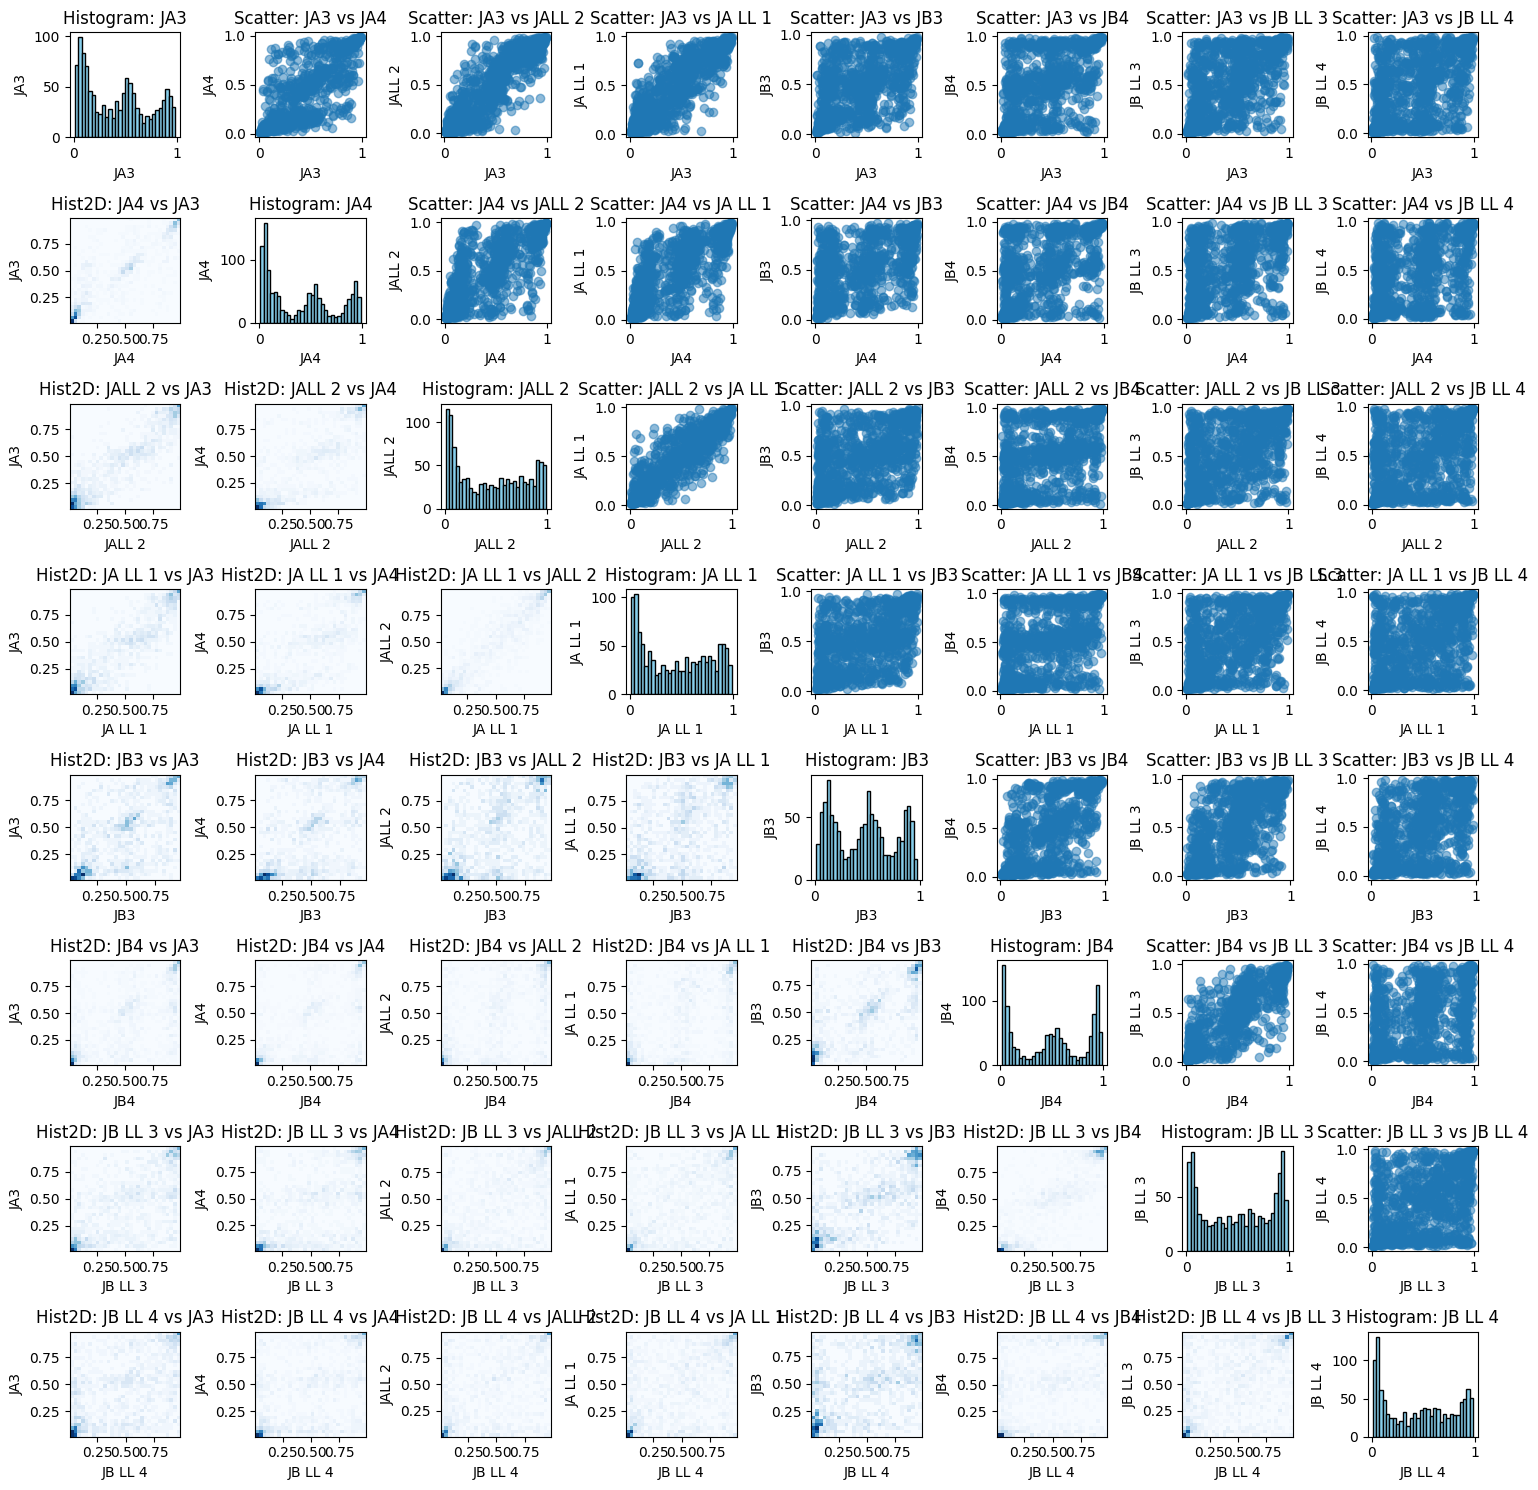
\includegraphics[width=\textwidth]{Chapter_5/figures/fCpG_loci_J.png}
\caption{Visualisation of fCpG arrays for patient J and the inter-gland
    correlation plots.}
\label{fig:vis_J}
\end{figure}

\begin{figure}[h]
\centering
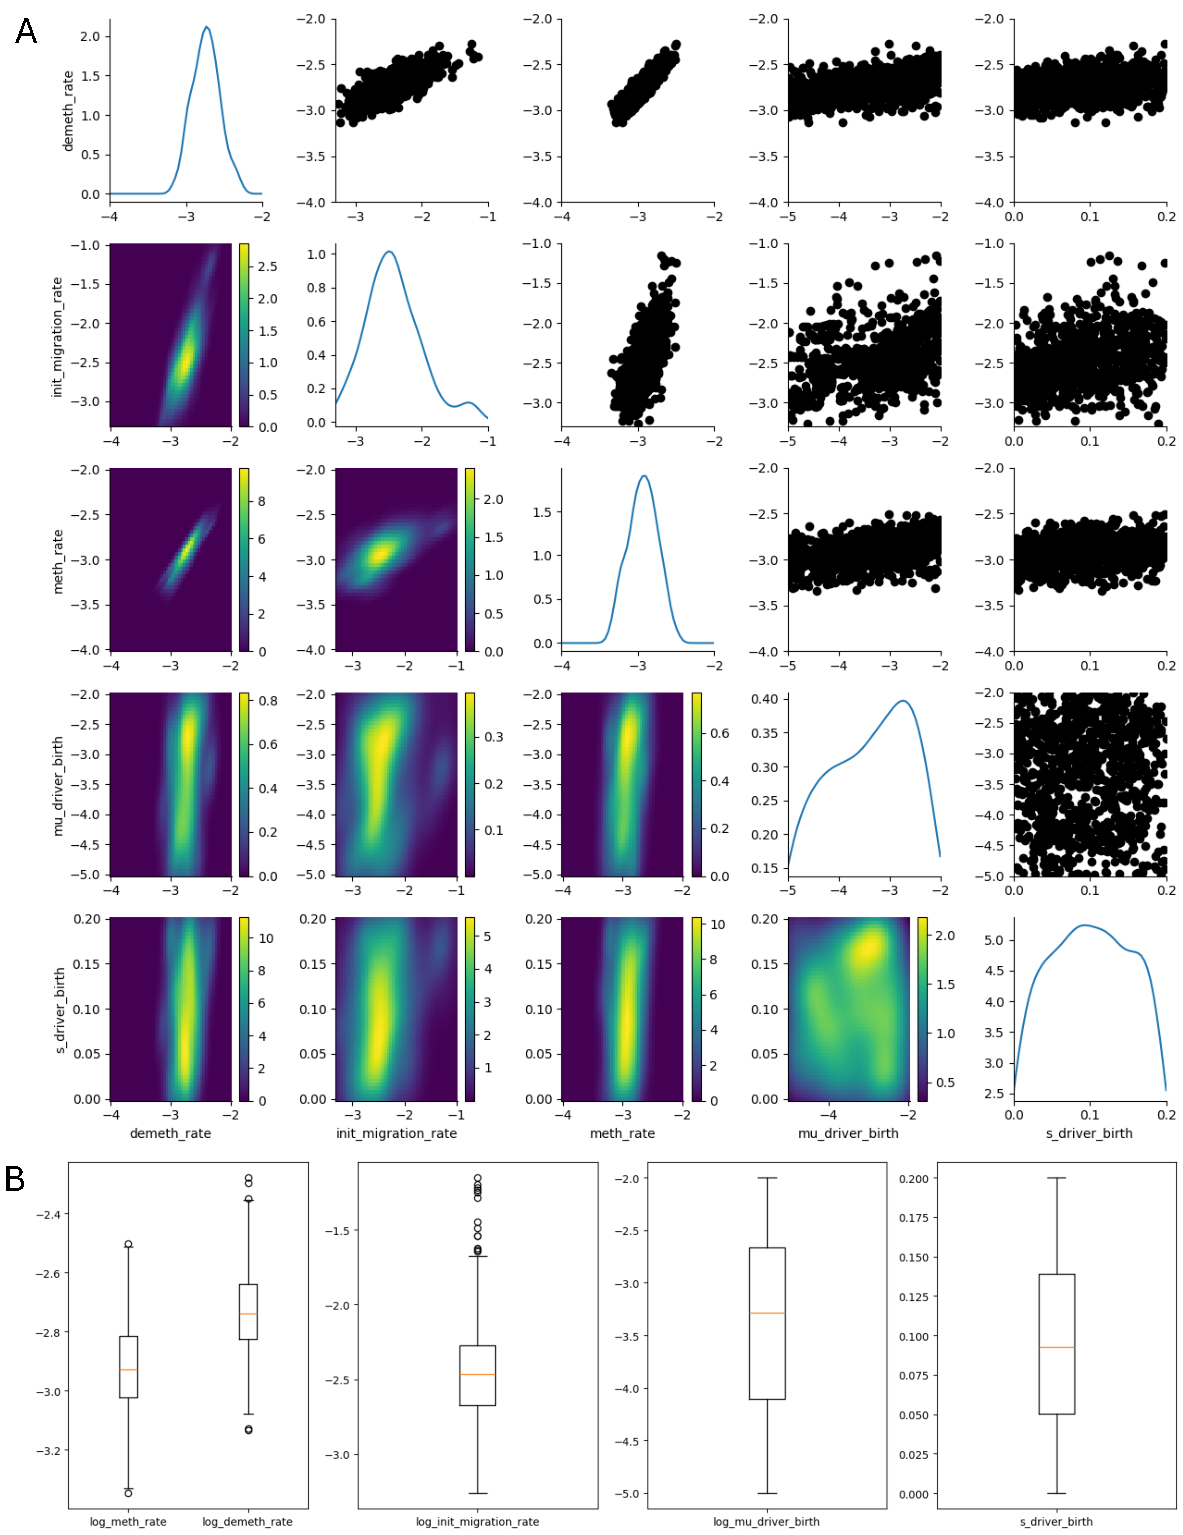
\includegraphics[width=\textwidth]{Chapter_5/figures/inference_J.pdf}
\caption{Inference of the parameters for patient J.}
\label{fig:inference_J}
\end{figure}

\begin{figure}[ht]
\centering
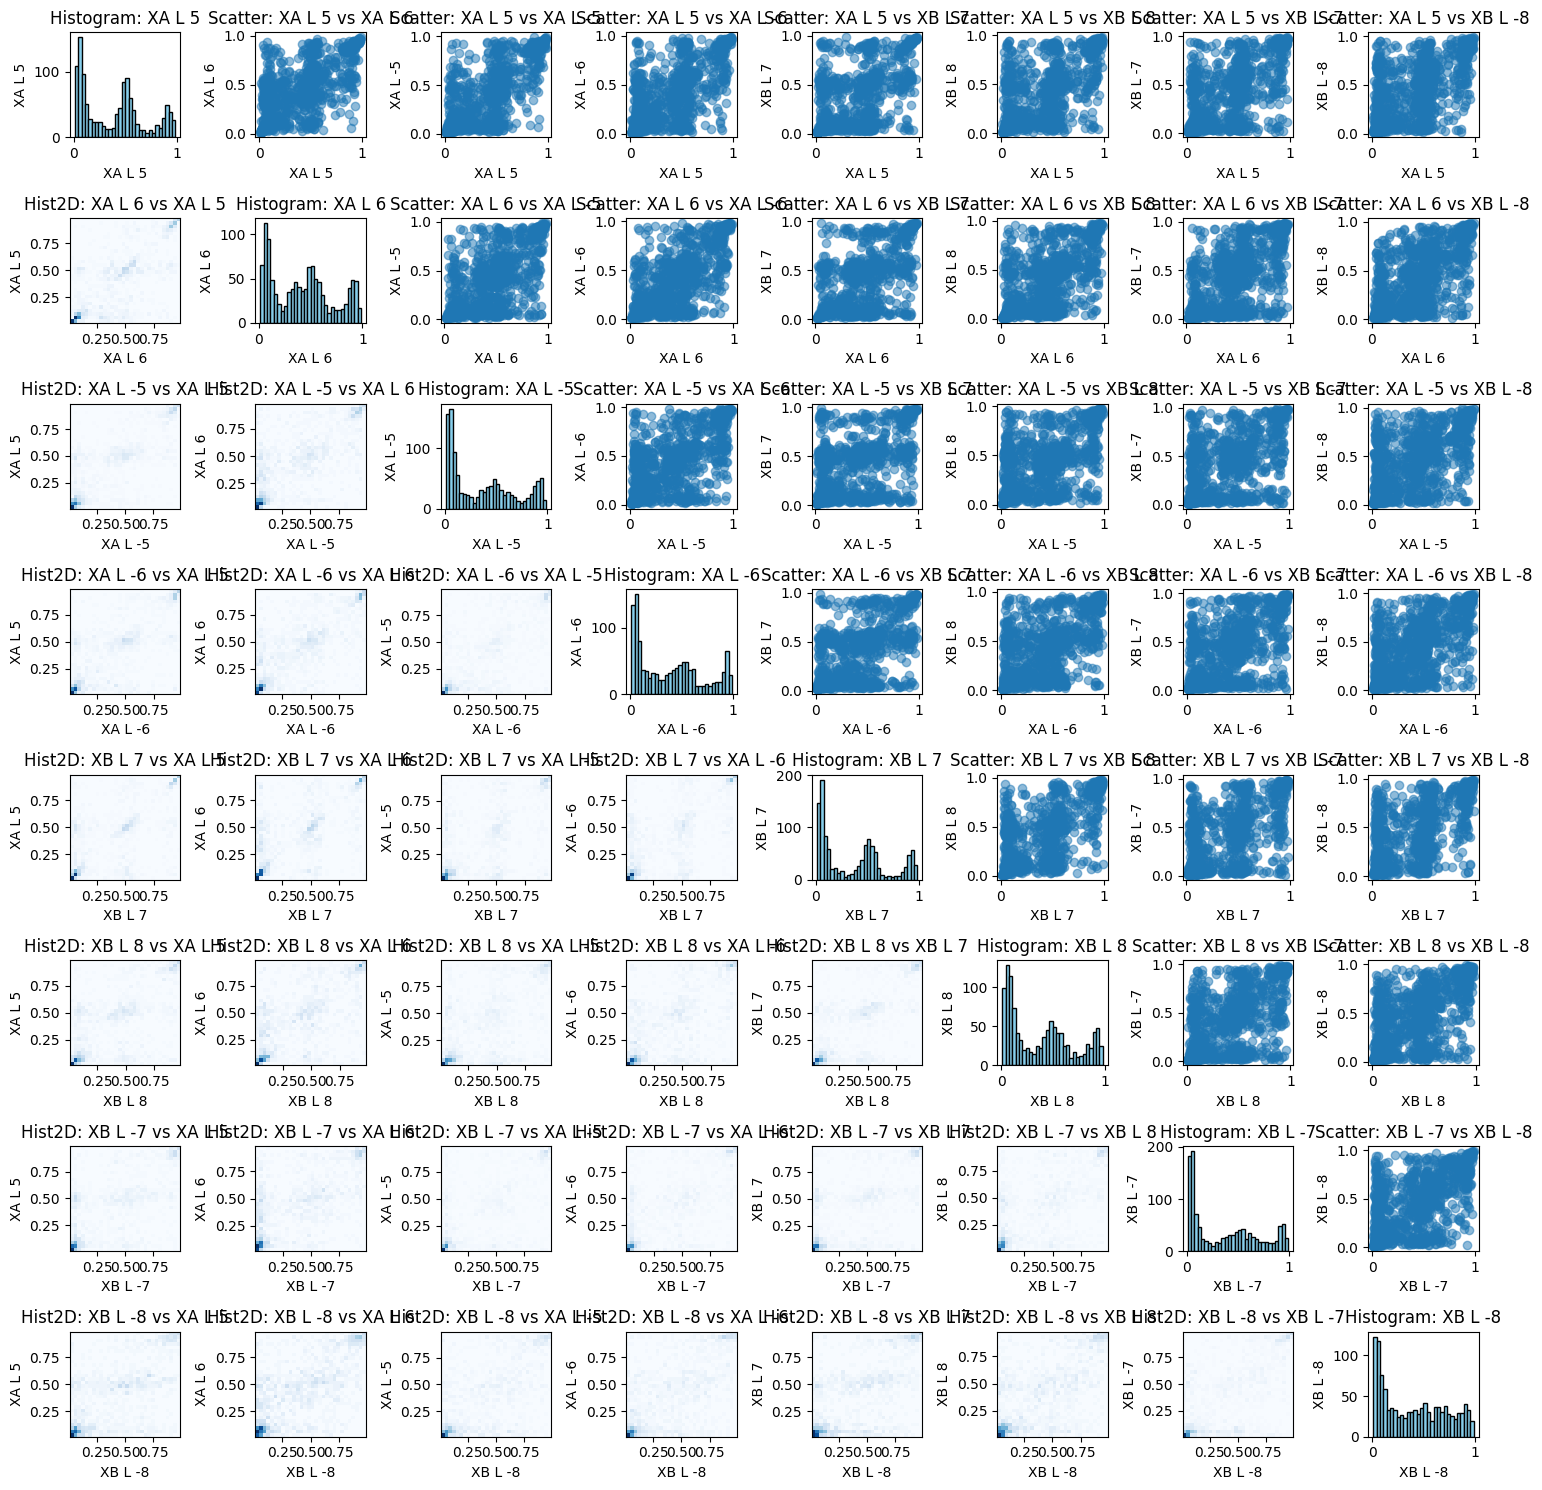
\includegraphics[width=\textwidth]{Chapter_5/figures/fCpG_loci_X.png}
\caption{Visualisation of fCpG arrays for patient X and the inter-gland
    correlation plots.}
\label{fig:vis_X}
\end{figure}

\begin{figure}[h]
\centering
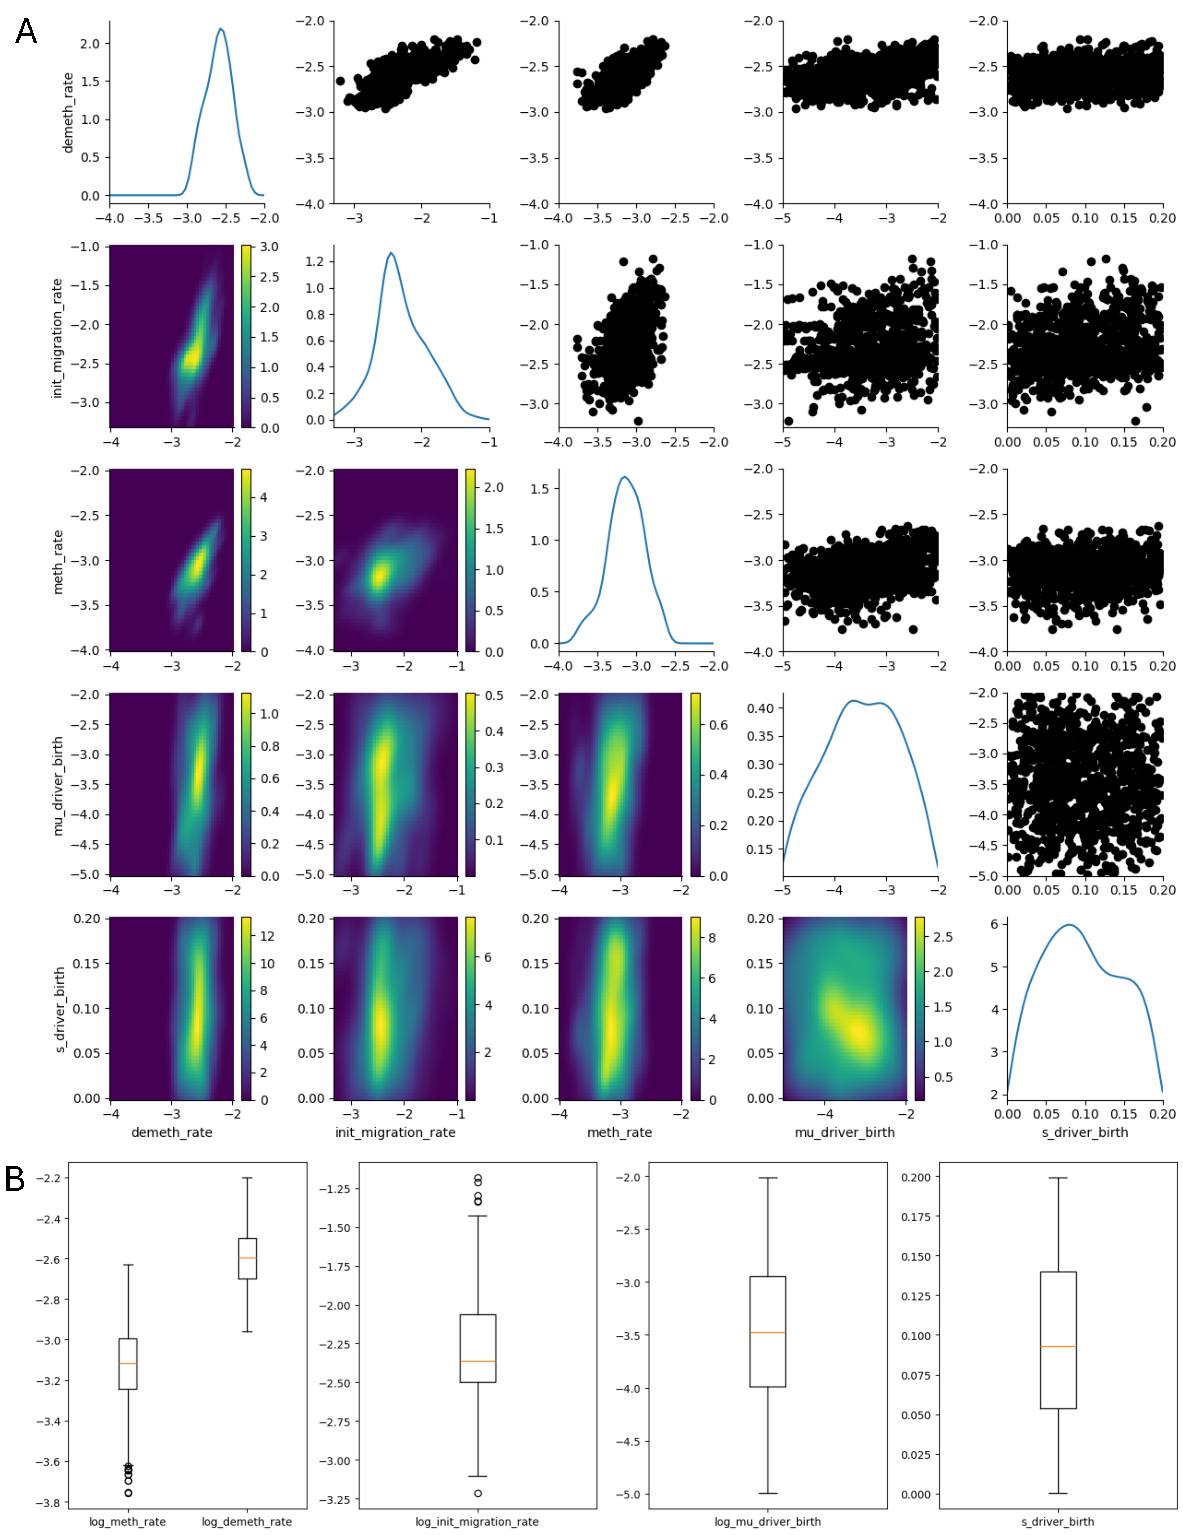
\includegraphics[width=\textwidth]{Chapter_5/figures/inference_X.pdf}
\caption{Inference of the parameters for patient X.}
\label{fig:inference_X}
\end{figure}

\begin{figure}[ht]
\centering
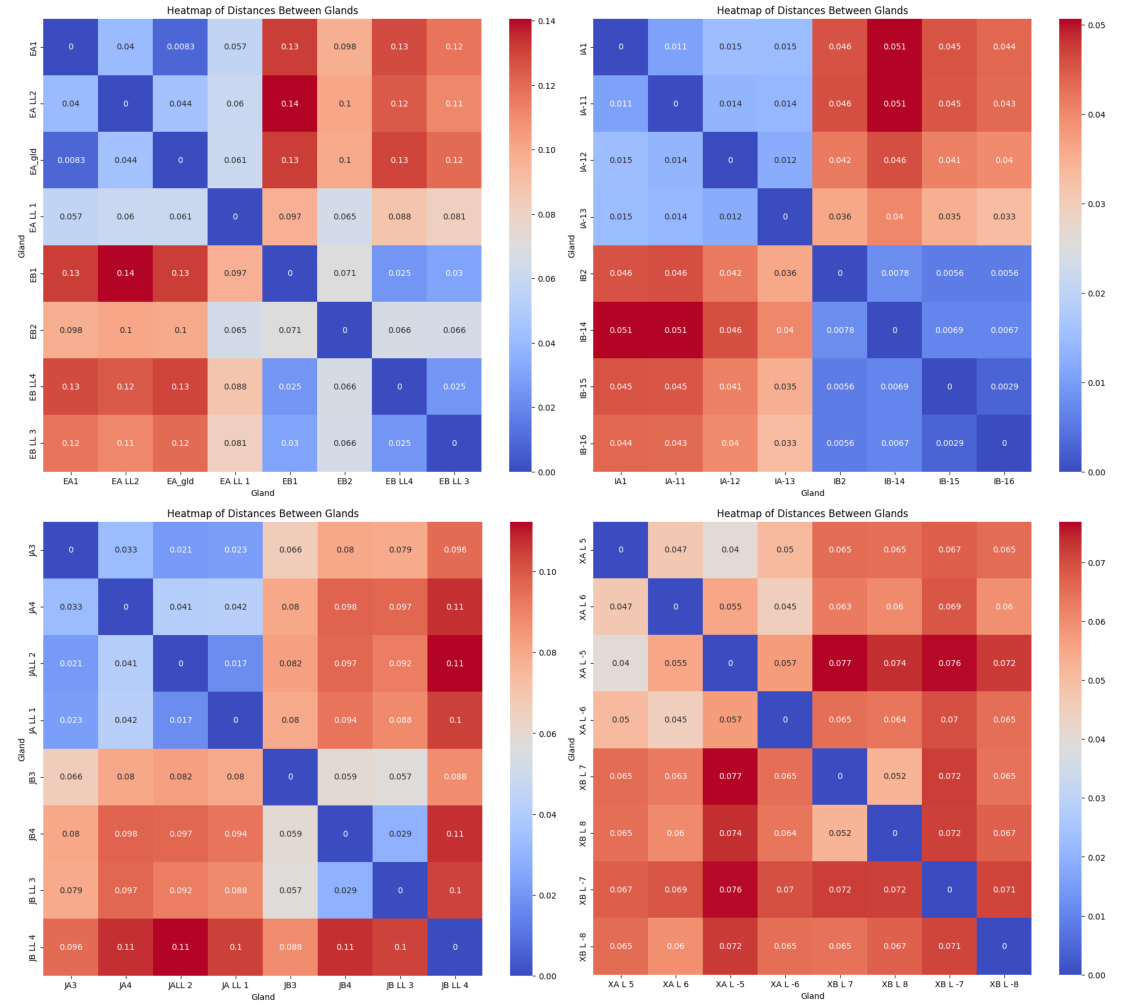
\includegraphics[width=\textwidth]{Chapter_5/figures/gland_dists.pdf}
\caption{Inter-gland distance matrices for the tumours modelled in this thesis.
    Clockwise from top left: E, I, X, J.}
\label{fig:gland_dists}
\end{figure}


%Contributions

%Coment after Contribution title:
\renewcommand{\bibpreamble}{The academic contributions made during the time this research was carried
out are listed below:}

\nocitectb{*}

\cleardoublepage
\phantomsection
\addcontentsline{toc}{chapter}{Contributions}
\bibliographystylectb{agsm}
\bibliographyctb{Bibliography/bbl_user}


%'multibib' package is used to generate the Contribution chapter as an extra bibliography chapter. When using multibib package on Windows it may fail. The solution is to run manually the following compilations:
%pdflatex Thesis.tex
%bibtex Thesis.tex
%bibtex ctb.aux	-> This file is created in the main folder after running the 'bibtex Thesis.tex' compilation.
%pdflatex thesis.tex
%pdflatex thesis.tex
%Check multibib documentation for more options. - https://www.ctan.org/pkg/multibib



%Bibliography
\renewcommand{\bibpreamble}{ } %No coments after bibliography title. It had been changed in Contributions.
\cleardoublepage
\phantomsection
\addcontentsline{toc}{chapter}{Bibliography}
\bibliographystyle{agsm}
\bibliography{Bibliography/zotero.bib}

\end{document}
